% Created 2023-10-30 Mon 15:15
% Intended LaTeX compiler: xelatex
\documentclass[aspectratio=1610, 10pt]{beamer}
\usepackage{graphicx}
\usepackage{grffile}
\usepackage{longtable}
\usepackage{wrapfig}
\usepackage{rotating}
\usepackage[normalem]{ulem}
\usepackage{amsmath}
\usepackage{textcomp}
\usepackage{amssymb}
\usepackage{amsthm}
\usepackage{capt-of}
\usepackage{hyperref}
\usepackage{geometry}
\usepackage{siunitx}
\usepackage{dsfont}
\usepackage{booktabs}
\usepackage[cache=false]{minted}
\usepackage{tcolorbox}
\usepackage{forest}
\usepackage{etoolbox}
\BeforeBeginEnvironment{minted}{\begin{tcolorbox}[colback=black,colframe=black]}%
\AfterEndEnvironment{minted}{\end{tcolorbox}}%
\usemintedstyle{native}
% Add support for \subsubsectionpage
\def\subsubsectionname{\translate{Subsubsection}}
\def\insertsubsubsectionnumber{\arabic{subsubsection}}
\setbeamertemplate{subsubsection page}
{
\begin{centering}
{\usebeamerfont{subsubsection name}\usebeamercolor[fg]{subsubsection name}\subsubsectionname~\insertsubsubsectionnumber}
\vskip1em\par
\begin{beamercolorbox}[sep=4pt,center]{part title}
\usebeamerfont{subsubsection title}\insertsubsubsection\par
\end{beamercolorbox}
\end{centering}
}
\def\subsubsectionpage{\usebeamertemplate*{subsubsection page}}

\AtBeginSection{\frame{\sectionpage}}
\AtBeginSubsection{\frame{\subsectionpage}}
\AtBeginSubsubsection{\frame{\subsubsectionpage}}
\usefonttheme[onlymath]{serif}
\AtBeginDocument{%
\DeclareSymbolFont{pureletters}{T1}{lmr}{\mddefault}{it}%
}
\DeclareMathOperator{\sgn}{sgn}
\usepackage{animate}
\usetheme{sigma}
\author{Aditya}
\date{}
\title{Low Density Parity Check Codes}
\subtitle{AKA Gallager Codes}
\hypersetup{
 pdfauthor={Aditya},
 pdftitle={Low Density Parity Check Codes},
 pdfkeywords={},
 pdfsubject={},
 pdfcreator={Emacs 28.2 (Org mode 9.5.5)},
 pdflang={English}}
\begin{document}

\maketitle
\begin{frame}{Outline}
\tableofcontents
\end{frame}



\section{Formalizing Error Correction Codes}
\label{sec:org2c6c725}

\begin{frame}[label={sec:orgd526036}]{The Model}
\begin{itemize}
\item Transmitter AKA modulator does bits \(\mapsto\) signals.
\item In our model, noise source adds Gaussian noise \(n(t)\) that is
independent from symbol to symbol.
\end{itemize}
\begin{center}
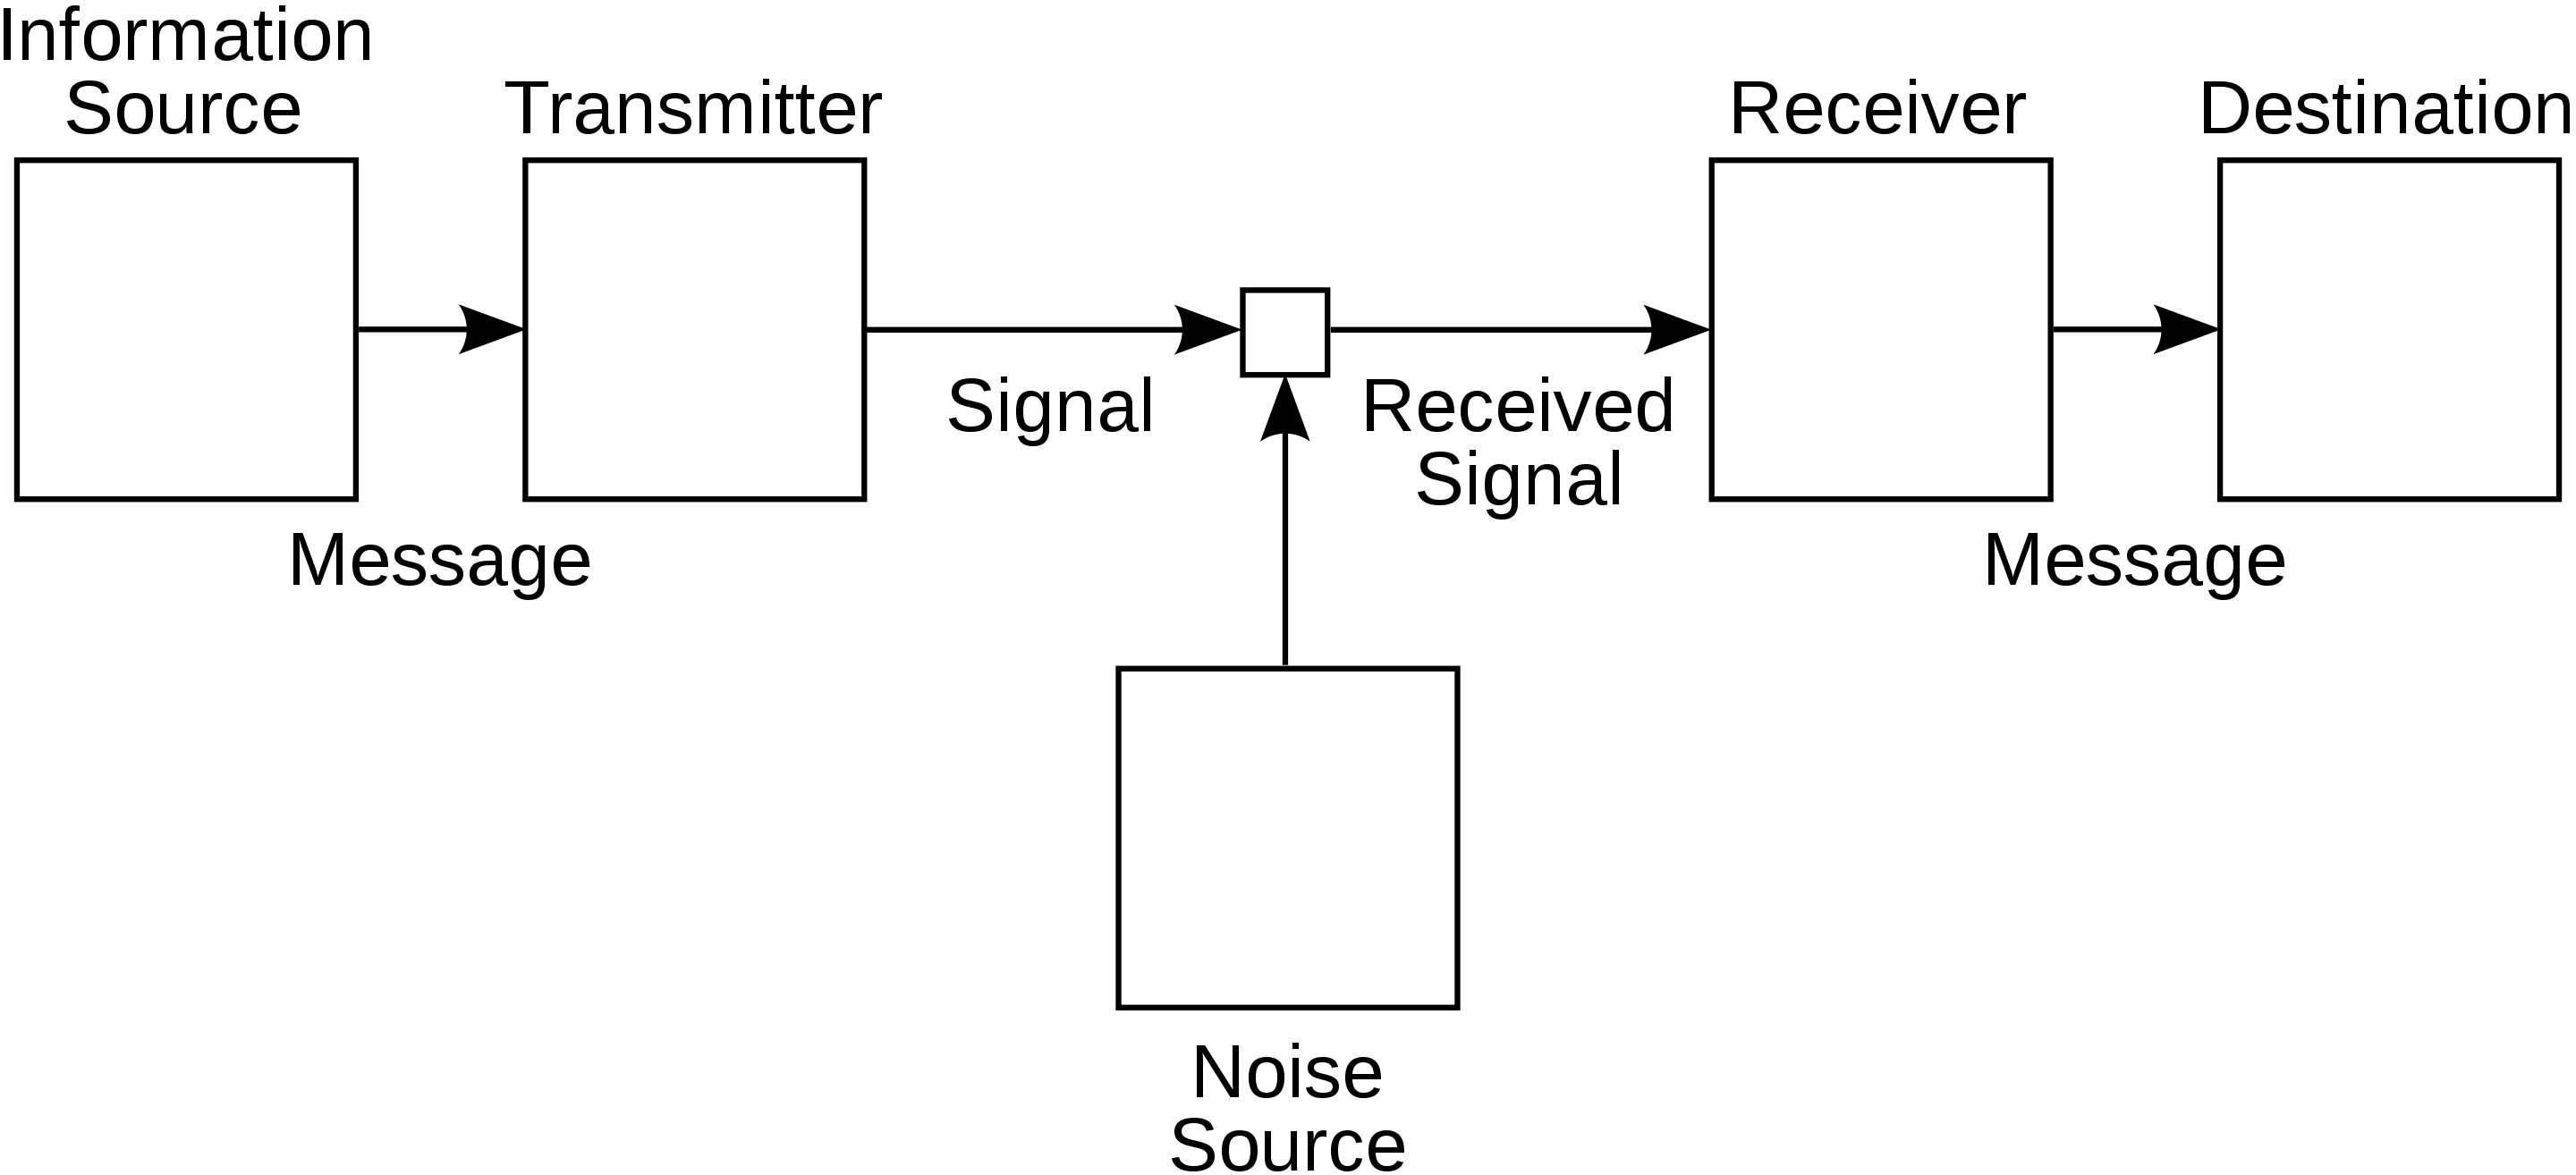
\includegraphics[width=.9\linewidth]{./shannon_gen_comm_sys.png}
\end{center}
\end{frame}

\begin{frame}[label={sec:orgba6f001}]{Modulation}
\begin{itemize}
\item Remember, the goal is to map bits (0s and 1s) to a signal.
\item We will use binary phase shift keying (BPSK), which works by
changing (\emph{modulating}) the phase of a basis function. Then,
\(0\mapsto s_0(t)\) and \(1\mapsto s_1(t)\):
\begin{align*}
s_0(t) &= \sqrt{\frac{2E}{T}} \sin{\left(2\pi ft + \frac{\pi}{2} \right)}\\
s_1(t) &= \sqrt{\frac{2E}{T}} \sin{\left(2\pi ft - \frac{\pi}{2} \right)}
\end{align*}
\item Looks hard, but phasors can help!
\end{itemize}
\end{frame}

\begin{frame}[label={sec:org2e34753}]{Constellations}
\begin{itemize}
\item Constellation diagram (very similar to phasor diagram) -- in
\(\mathbb{C}\), the argument gives the phase shift, and the norm gives
the amplitude of a signal.
\begin{center}
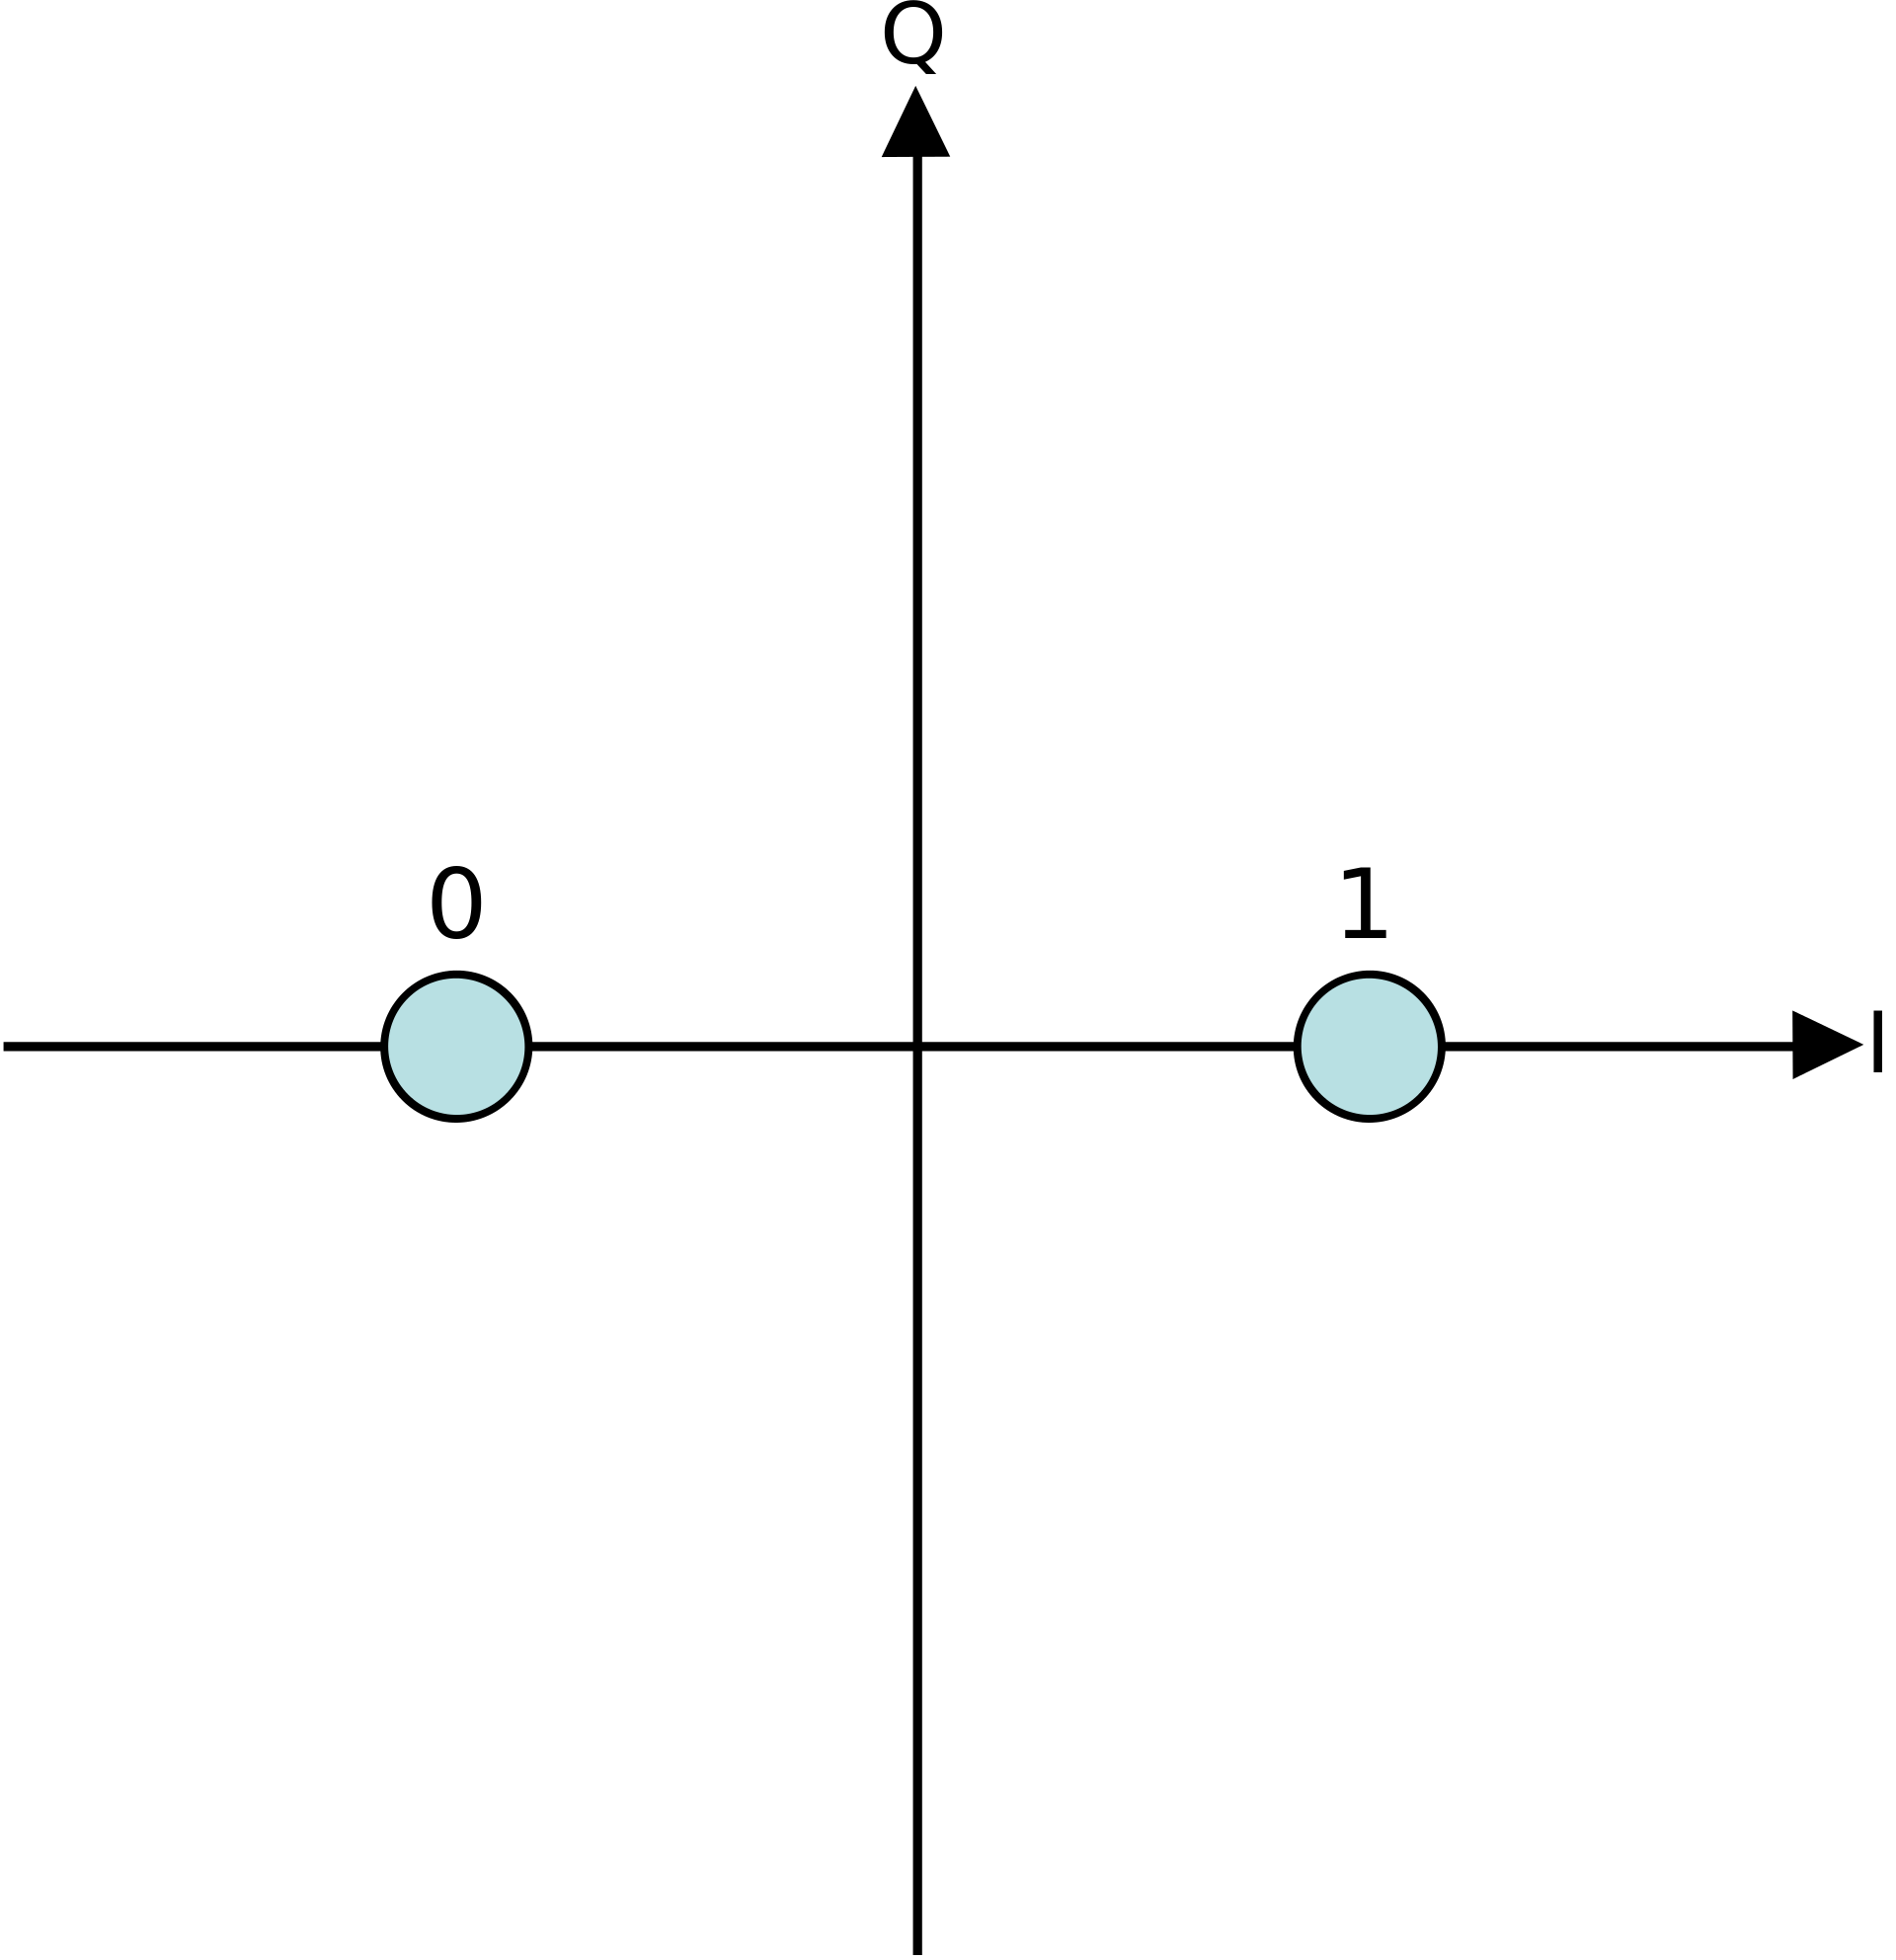
\includegraphics[width=0.25\textwidth]{./bpsk_const.png}
\end{center}
\item So, BPSK maps \(0\mapsto +1\) and \(1\mapsto -1\). Note that this is a
mapping from \(\mathbb{F}_2 \mapsto \mathbb{R}\).
\end{itemize}
\end{frame}

\begin{frame}[label={sec:org3e3f3d9}]{BPSK in time domain}
\begin{center}
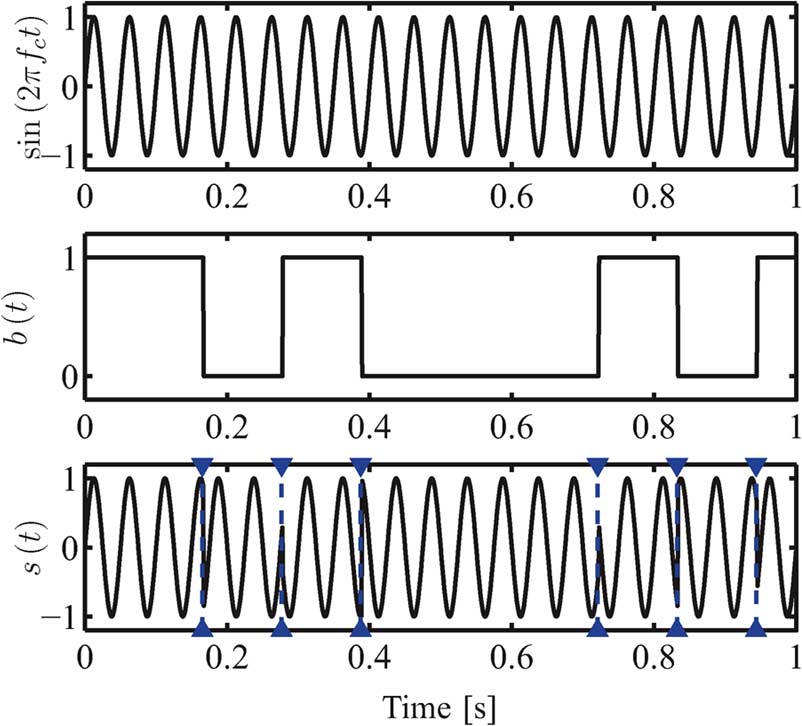
\includegraphics[width=0.5\textwidth]{./bpsk_time_domain.png}
\end{center}
\end{frame}

\begin{frame}[label={sec:org776ca90}]{Through the channel}
We add in white Gaussian noise (AWGN).
$$y(t) = x(t) + n(t)$$
where \(x(t)\) is the input signal, and \(n(t)\) is a Gaussian process,
and independent for each symbol.
\end{frame}

\begin{frame}[label={sec:org55de732}]{Demodulate!}
$$\rho = \int_0^T y(t) \sqrt{\frac{2E}{T}}\sin{\left(2\pi ft +
\frac{\pi}{2} \right)} dt$$

\begin{itemize}
\item \alert{Important:} \(\rho\in\mathbb{R}\).
\item Why does this work? There's a little bit of analog signal processing
that's not too relevant\ldots{}in essence, the process involves
re-multiplying by the carrier signal, then using a low pass filter
to pick out the data.
\end{itemize}
\end{frame}

\begin{frame}[label={sec:orgc6ca06b}]{What do we do with \(\rho\)?}
Remember, we need to map back from \(\mathbb{R} \mapsto \mathbb{F}_2\).

\alert{Hard decision decoding:} Threshold at 0 to get the output bit:

$$b = \begin{cases} 0,& \rho > 0\\ 1,&\rho \leq 0\end{cases}$$

\alert{Soft decision decoding:} We'll talk about it soon!
\end{frame}

\begin{frame}[label={sec:orge9163c1}]{Binary symmetric channels}
\begin{itemize}
\item It can be shown that BPSK over AWGN is a BSC.
\end{itemize}

\begin{center}
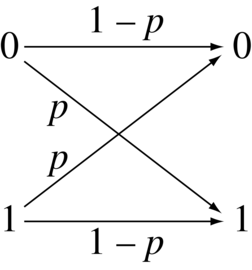
\includegraphics[width=0.2\textwidth]{./bsc.png}
\end{center}
\end{frame}

\begin{frame}[label={sec:org537066a}]{How to compute bit-flip probability \(p\)?}
The bit-error rate \(p\) is given by:
$$\text{BER} = P(t = +1)\cdot P(n \leq -1) + P(t = -1)\cdot P(n \geq +1)$$
Assuming an even mix of 0s and 1s,
$$\text{BER} = \frac{1}{2} P(n \leq -1) + \frac{1}{2} P(n \geq +1)$$
Recall, the noise is a Gaussian distribution with variance \(\sigma\).
\end{frame}

\begin{frame}[label={sec:orgc599a74}]{After some statistics\ldots{}}
The transition probability of our model is:
$$p = \text{BER} = Q\left(\frac{1}{\sigma} \right)$$
\begin{center}
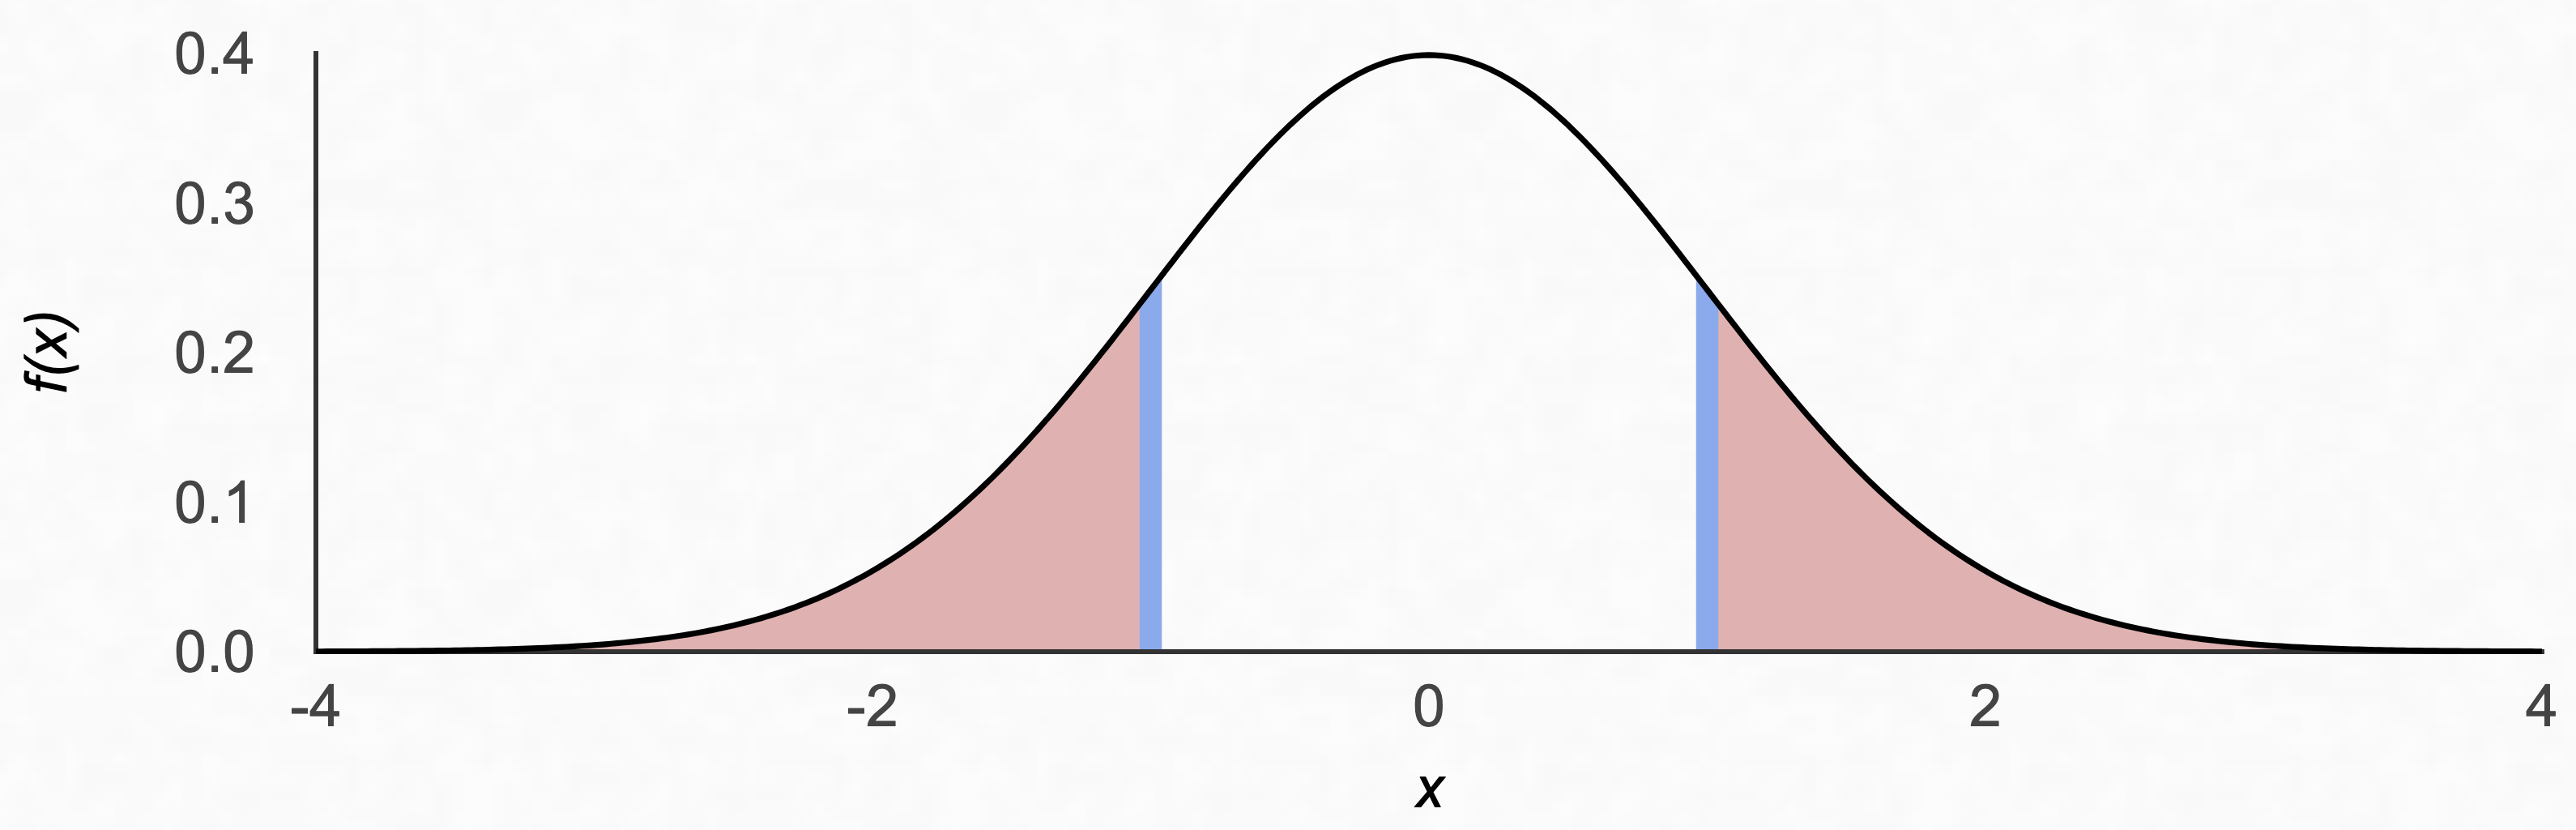
\includegraphics[width=.9\linewidth]{./gaussian_twoside.png}
\end{center}
$$Q(x) := \frac{1}{2} \text{erfc}\left(\frac{x}{\sqrt{2}} \right)$$
\end{frame}

\begin{frame}[label={sec:org69ff48d}]{One last thing: power!}
Signal-to-noise ratio:
$$\mathrm{SNR_{dB}} = 10\log_{10}{\left(\frac{P_{\text{signal}}}{P_{\text{noise}}} \right)}$$

In discrete time,
$$\text{SNR} = \frac{E_s}{\sigma^2} = \frac{E_s}{\frac{N_0}{2}} = \frac{2E_s}{N_0}$$
where \(E_s\) is the energy per symbol, \(N_0/2\) is the power spectral
density (variance) of the noise signal.
\end{frame}

\begin{frame}[label={sec:orgb4d8724}]{SNR for BPSK}
$$E_s = \frac{(-1)^2 + 1^2}{2} = 1\implies \text{SNR} =
\frac{1}{\sigma^2}$$

We get a nice relation between SNR and BER for our model:
$$\text{BER} = Q\left(\sqrt{\text{SNR}}\right)$$
\end{frame}

\begin{frame}[label={sec:org2489d81}]{SNR vs. BER}
Red line is a Monte-Carlo simulation that counts bit errors for AWGN
(\(\sigma = 1\)).We usually use \(E_b/N_0\) (SNR per bit) instead of
\(2E_s/N_0\) (SNR) in these graphs.
\begin{center}
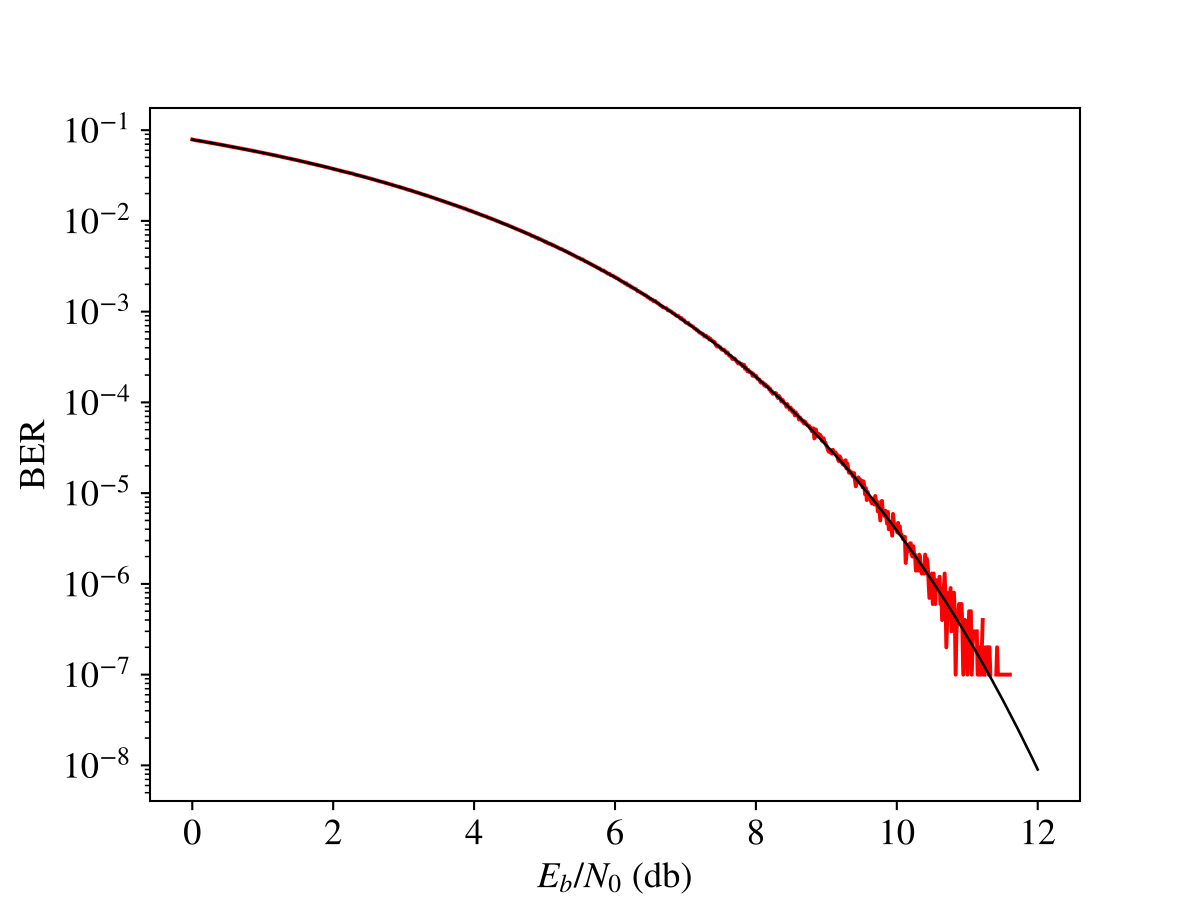
\includegraphics[width=0.6\textwidth]{./snr_ber_plot.png}
\end{center}
\end{frame}

\begin{frame}[label={sec:org3610f89}]{What do error correction codes do?}
\begin{center}
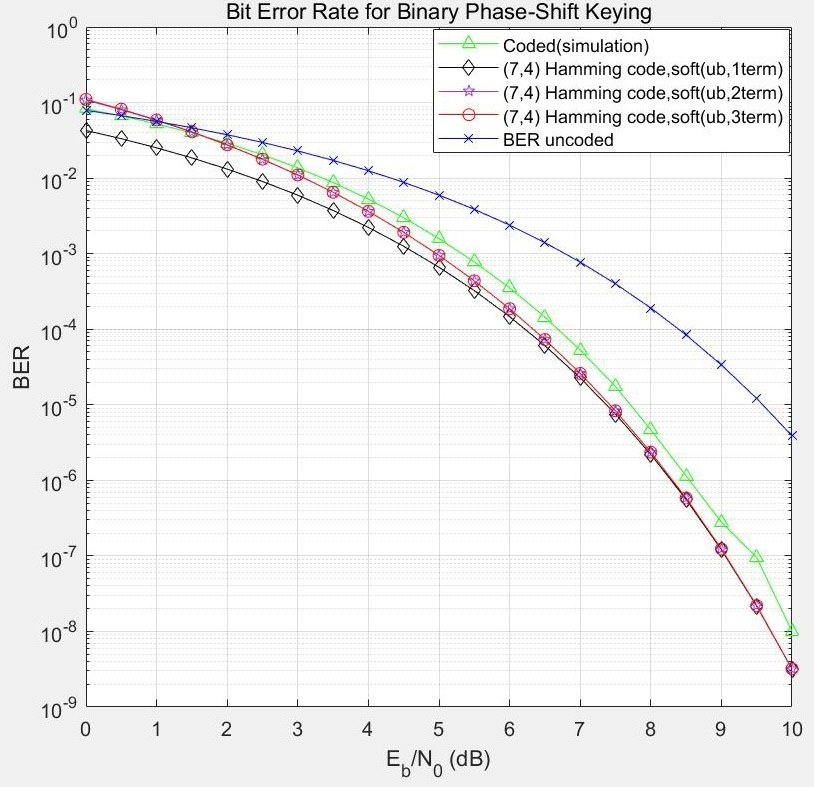
\includegraphics[width=0.6\textwidth]{./error_correction_ber_snr.jpeg}
\end{center}
\end{frame}

\begin{frame}[label={sec:orgc077cf1}]{Shannon Limit and Capacity-Approaching Codes}
\(E_b = E_s/R = nE_s/k\)
\begin{center}
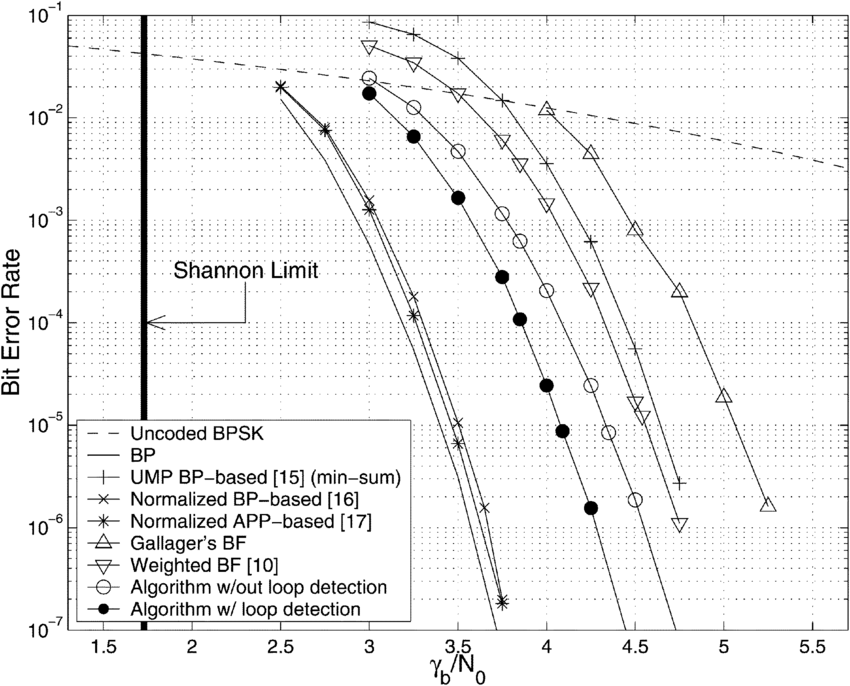
\includegraphics[width=0.7\textwidth]{./ldpc_ber_snr.png}
\end{center}
\end{frame}

\section{Simple Soft Decision Decoders}
\label{sec:orgb68b010}

\begin{frame}[label={sec:org3c74cf0}]{\(n=3\) Repetition Code}
What's the easiest way to make sure someone understands \emph{exactly} what
you're saying?\\

Repeat yourself (say it three times)!
\end{frame}

\begin{frame}[label={sec:org8a1352f},fragile]{Encoder}
 Note that the rate of this code is \(k/n = 1/3\).
\begin{center}
\begin{tabular}{ccccccc}
\toprule
\(m\) & \(c\) & \(\vec{s}\)\\
\midrule
0 & 000 & \texttt{[+1, +1, +1]}\\
1 & 111 & \texttt{[-1, -1, -1]}\\
\bottomrule
\end{tabular}

\end{center}
\end{frame}

\begin{frame}[label={sec:org8ba14ad}]{Hard decision decoder}
The output from the demodulator is some vector of real numbers,
say \(\vec{r} = [r_0, r_1, r_2]\). Then, hard decision decode this to
\(\vec{b}\) by thresholding at zero. Finally, use a majority function:

\begin{center}
\begin{tabular}{cc}
\toprule
\(\vec{b}\) & \(\hat{c}\)\\
\midrule
000 & 000\\
001 & 000\\
010 & 000\\
100 & 000\\
\midrule
011 & 111\\
101 & 111\\
110 & 111\\
111 & 111\\
\bottomrule
\end{tabular}

\end{center}
\end{frame}

\begin{frame}[label={sec:org119ada6}]{So, we're happy with ourselves}
\begin{itemize}
\item Not so fast -- let's analyze this code within the formal framework
we laid out earlier.
$$\frac{E_b}{N_0} = \frac{E_s/\sigma^2}{2R} = \frac{3}{2\sigma^2}$$
\item The probability of a bit-flip is then:
$$\implies p = Q\left(\sqrt{\frac{2E_b}{3N_0}} \right)$$
\item The overall probability of an error is \(\text{BER} = 3p^2(1-p) +
  p^3\).
\end{itemize}
\end{frame}

\begin{frame}[label={sec:org0c26db0}]{Plotting the hard decision decoder for \(n=3\) repetition code}
\begin{center}
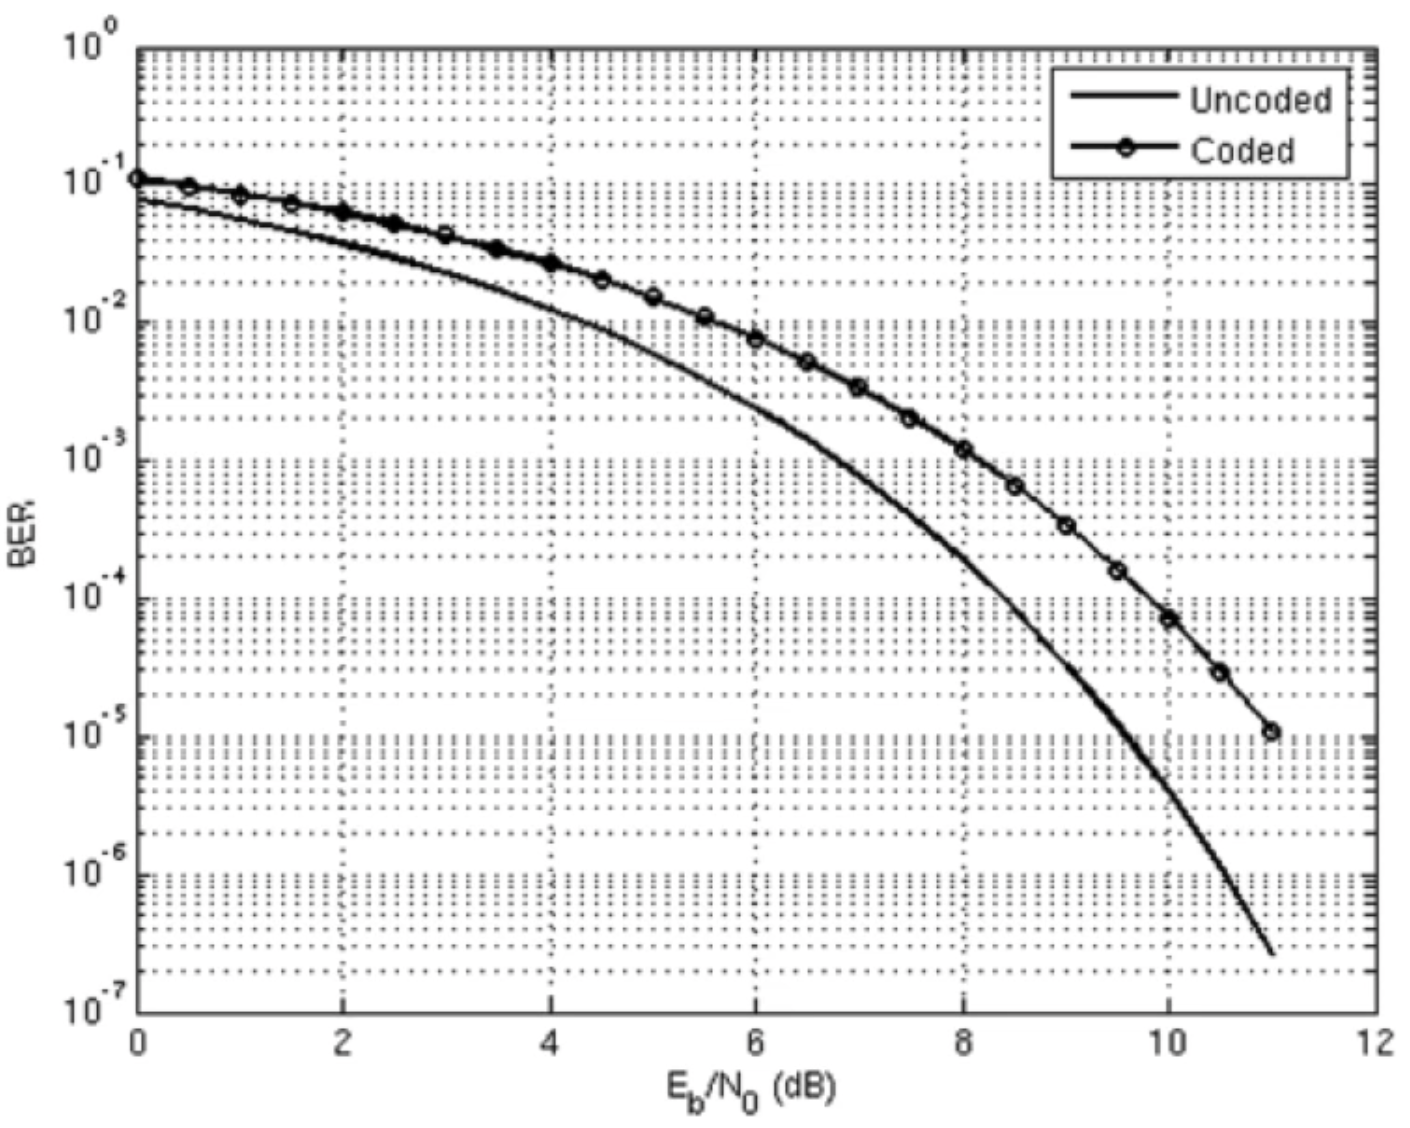
\includegraphics[width=0.6\textwidth]{./repetition_ber_snr.png}
\end{center}
\end{frame}

\begin{frame}[label={sec:org8cc8c79}]{Soft decision decoding}
\begin{itemize}
\item The received real vector \(\vec{r}\) can be analyzed in a real vector
space.
\item Compare the correlation of \(\vec{r}\) with the codewords, and pick
the output symbol based on that. If:
$$\vec{r} \cdot \begin{bmatrix} +1 & +1 & +1 \end{bmatrix} > \vec{r}
  \cdot  \begin{bmatrix} -1 & -1 & -1 \end{bmatrix}$$
\(\hat{c} = 000\) else \(\hat{c} = 111\).
\item More simply, check \(r_0 + r_1 + r_2 > 0\).
\item This is an optimal \alert{maximum likelihood decoder}.
\end{itemize}
\end{frame}

\begin{frame}[label={sec:orgd350f0d}]{BER vs SNR per bit for optimal decoding of repetition code}
\begin{center}
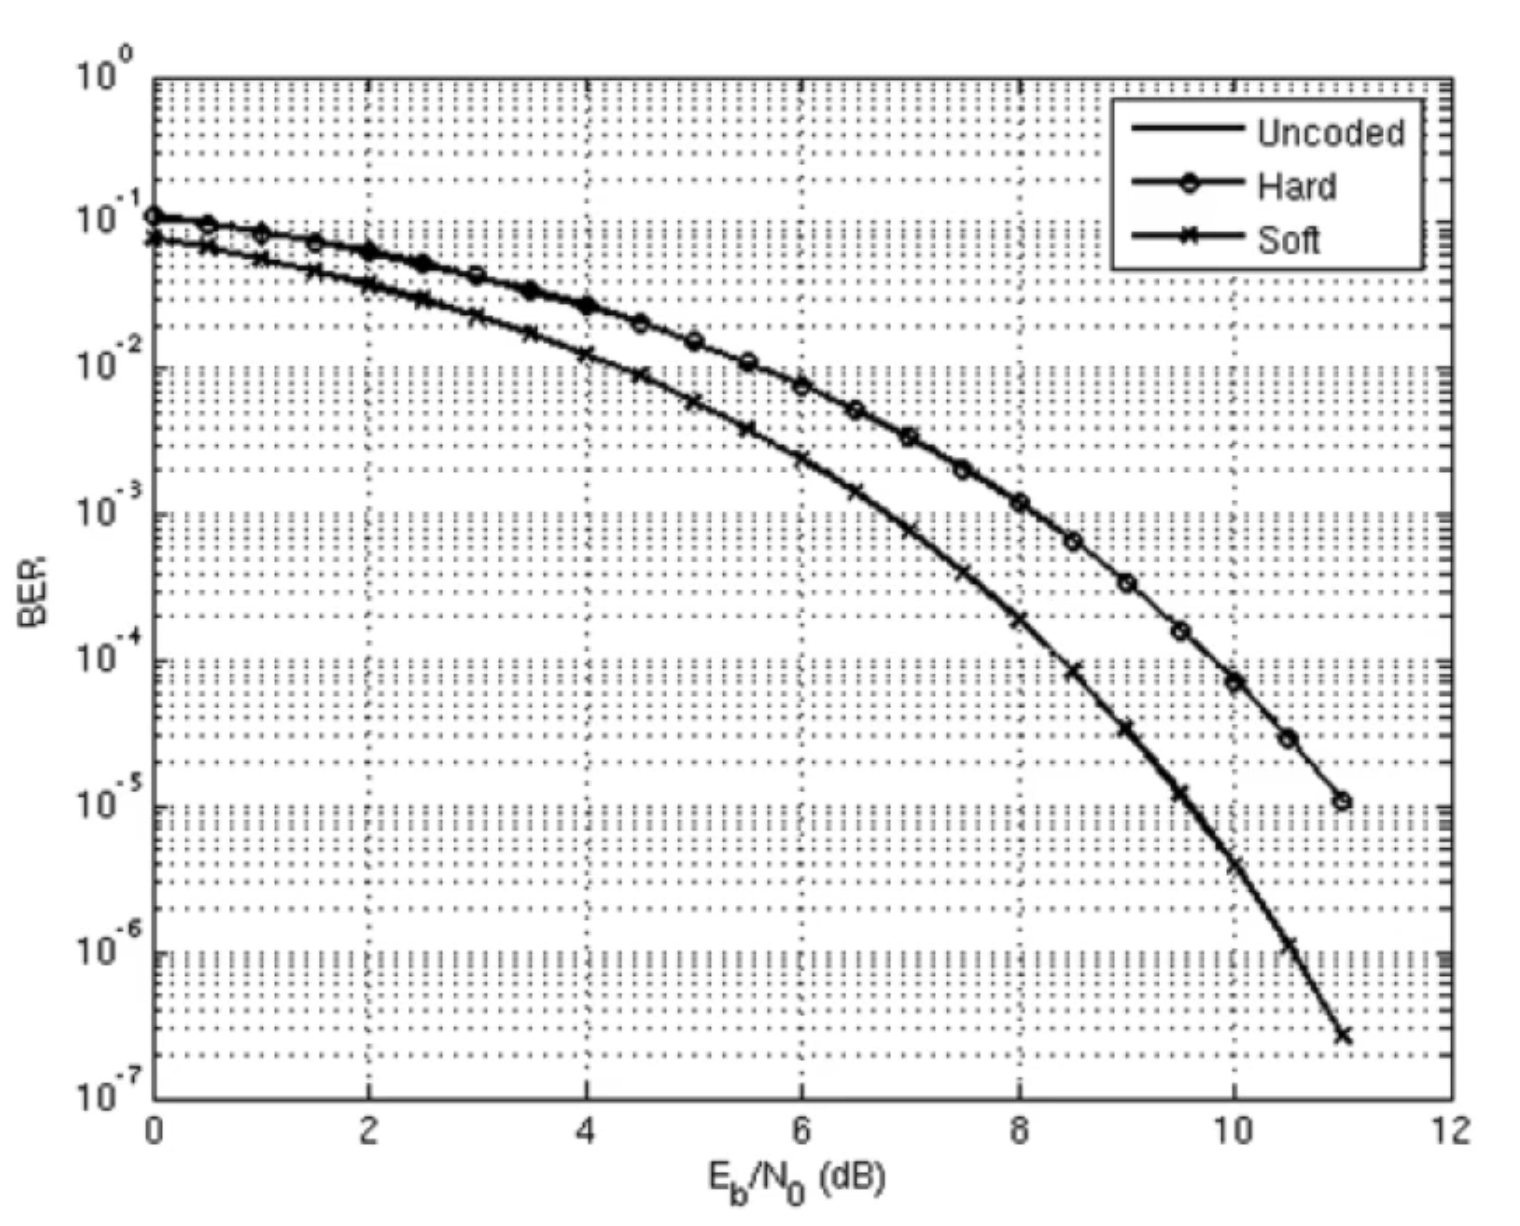
\includegraphics[width=0.6\textwidth]{./repetition_soft_ber_snr.png}
\end{center}
\end{frame}

\begin{frame}[label={sec:org72826eb}]{(7, 4) Hamming Code}
Recall from Anakin's introductory meeting on codes the (7, 4)
Hamming code.

\begin{center}
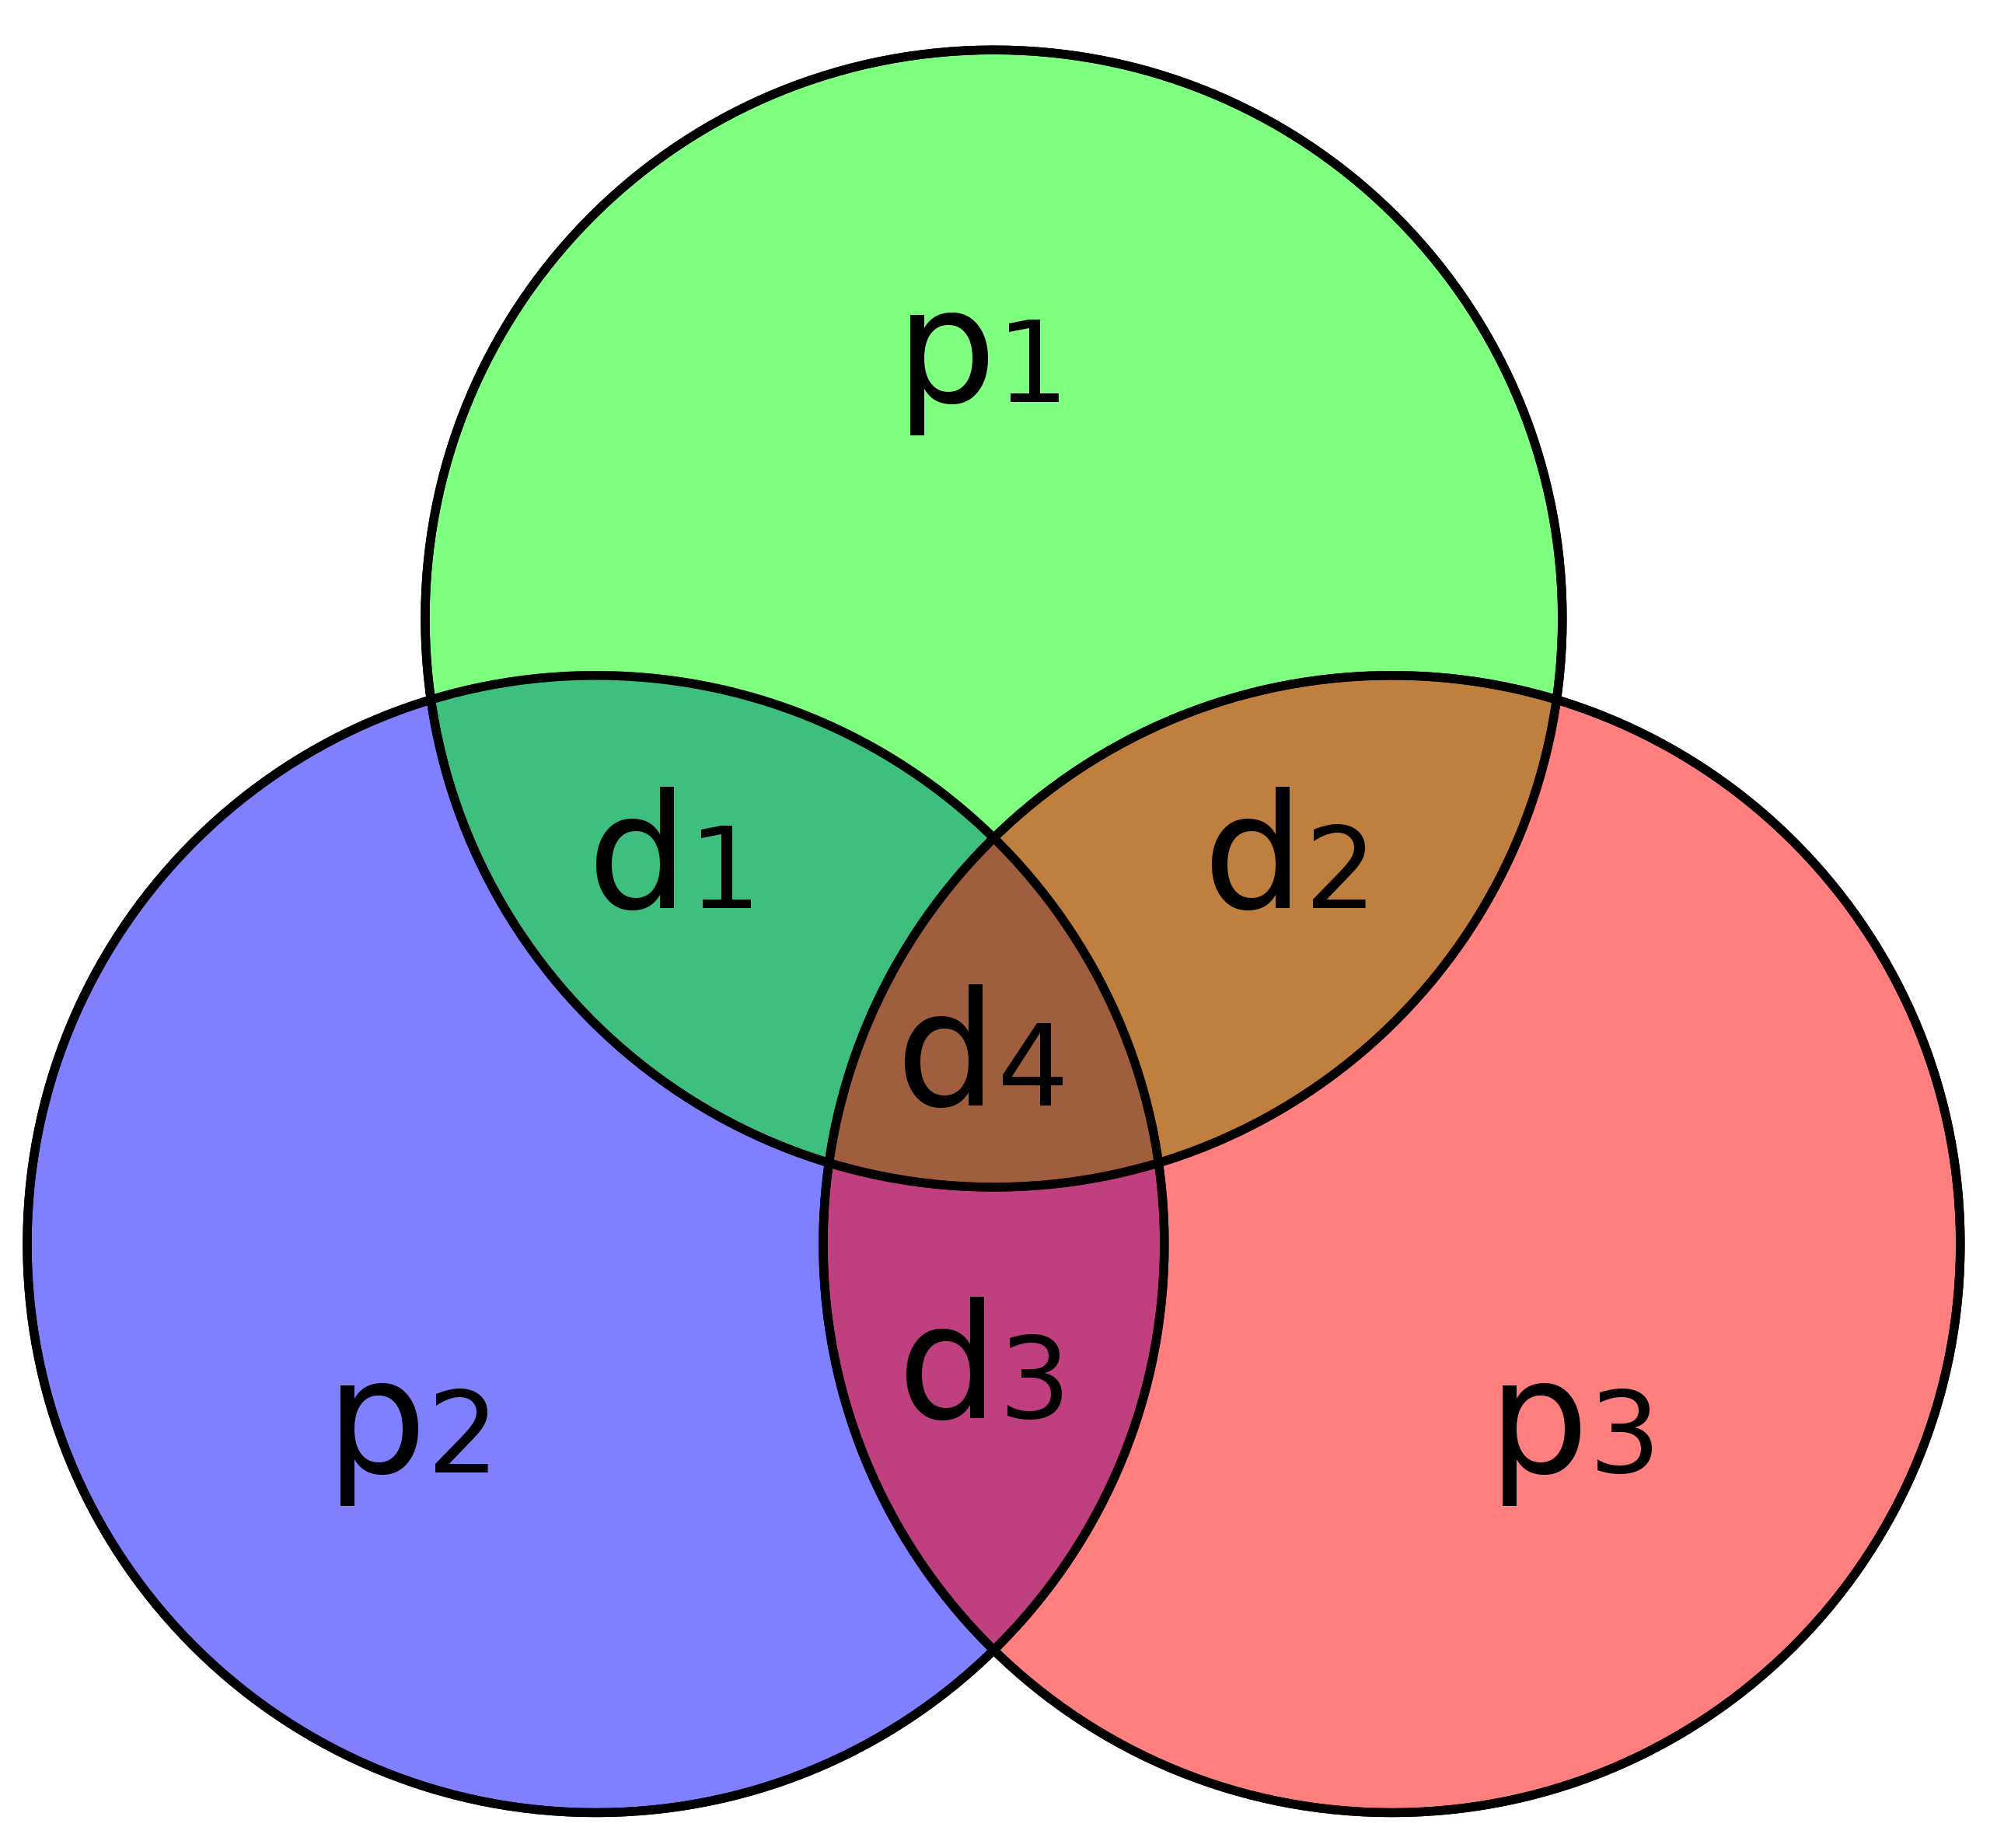
\includegraphics[width=0.5\textwidth]{./hamming74.png}
\end{center}
\end{frame}

\begin{frame}[label={sec:org714a7df}]{Hard decision decoder}
\begin{itemize}
\item \emph{After} the hard decision thresholding of the received vector
\(\vec{r}\) around 0 to get \(\vec{b}\),
\item Correct to the codeword at the closest Hamming distance from
\(\vec{b}\).
\item This is the \emph{minimum distance decoder} for the Hamming code.
\end{itemize}
\end{frame}

\begin{frame}[label={sec:org0f63d65}]{Soft decision decoder}
\begin{itemize}
\item Find the closest codeword to \(\vec{r}\) in \emph{Euclidean} distance.
\item That is, in the vector space \(\mathbb{R}^n\).
\item Clearly, this is (much) more complex, and becomes hard to implement
as \(k\) increases for a Hamming code.
\item This is the \emph{maximum likelihood decoder} for the Hamming code.
\end{itemize}
\end{frame}

\begin{frame}[label={sec:orge80b702}]{BER vs SNR per bit for Hamming (7,4) Decoders}
\begin{center}
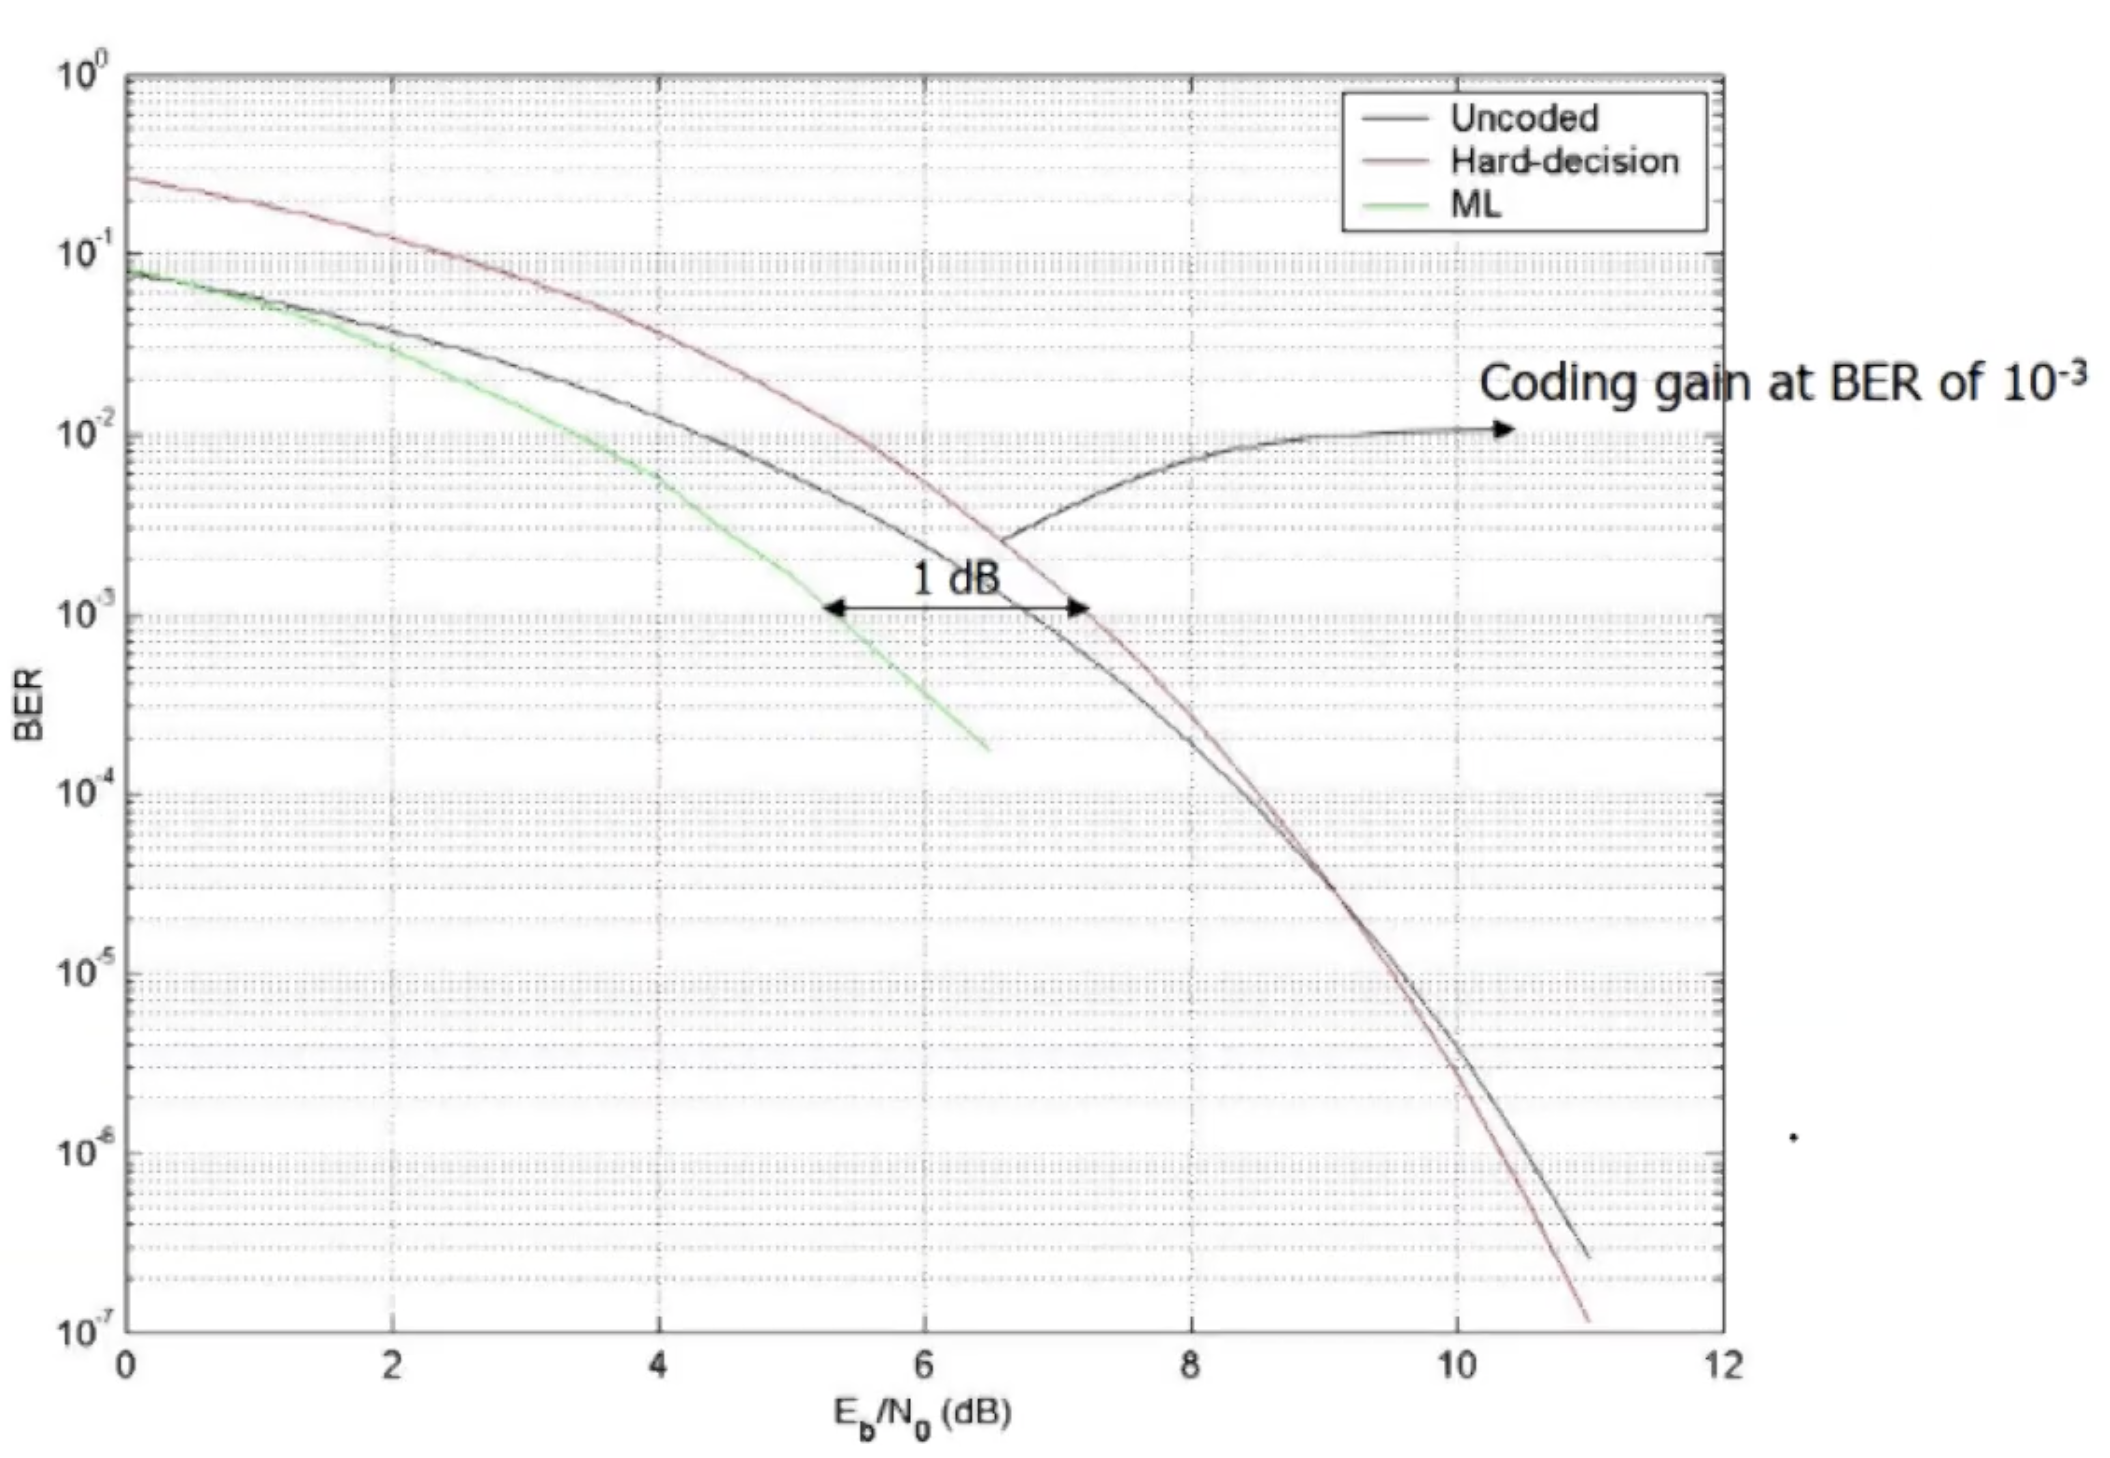
\includegraphics[width=0.75\textwidth]{./hamming_ber_snr.png}
\end{center}
\end{frame}

\begin{frame}[label={sec:orgef90246}]{SISO Decoding}
\begin{itemize}
\item There is another kind of decoder, the soft-in soft-out decoder.
\item We start with implementing it for the repetition code (this is
really easy and just for demonstrating the technique).
\end{itemize}
\end{frame}

\begin{frame}[label={sec:org4ad3b76}]{Belief}
\begin{itemize}
\item The output of the SISO decoder is a real vector \(\vec{L} =
  [L_{0}~L_1~L_2]\), where each \(L_i\) indicates the strength of the ``belief''
that bit \(c_i\) of the codeword is (say) 0.
\item What does this mean? Imagine you received the vector \([3.2,~4.3,~2.4]\).
\item This indicates that it's very likely, in each case, that the
transmitted symbol was \(+1\).
\end{itemize}
\end{frame}

\begin{frame}[label={sec:org52e8b01}]{Tell me more about your beliefs}
\begin{itemize}
\item What about \(\vec{r} = [0.02,~-3.2,~-0.6]\)?
\item A hard-decision decoder would turn this into \([1,~-1,~-1]\).
\item However, for a SISO decoder and a repetition code, you \emph{know} that
all the bits should be the same.
\item How sure are you about 0.02?
\end{itemize}
\end{frame}

\begin{frame}[label={sec:orgfb00f02}]{Formalizing the intuition}
The probabilities below are of interest (Bayes' rule):
$$P(c_0=0 | r_0) = \frac{f(r_0 | c_0=0)P(c_0=0)}{f(r_0)}$$
$$P(c_0=1 | r_0) = \frac{f(r_0 | c_0=1)P(c_0=1)}{f(r_0)}$$

It is natural to divide these quantities:
$$\frac{P(c_0=0 | r_0)}{P(c_0=1 | r_0)} = \frac{f(r_0 |
c_0=0)}{f(r_0 | c_0=1)}$$
\end{frame}

\begin{frame}[label={sec:org1fce1da}]{Intrinsic log likelihood ratios}
Recall that the noise is normally distributed, so \(f(r_0|c_0=0) = 1 +
N(0, \sigma^2)\) and \(f(r_0|c_0=1)= -1 + N(0, \sigma^2)\). Plugging in
the Gaussian PDF and simplifying gives
$$\frac{P(c_0=0 | r_0)}{P(c_0=1 | r_0)} = \exp{\frac{2r_0}{\sigma^2}}$$

So, the \emph{intrinsic log likelihood ratio} of \(r_0\) is:
$$l_0 = \log{\frac{P(c_0=0 | r_0)}{P(c_0=1 | r_0)}} = \frac{2r_0}{\sigma^2}$$
This is general for any intrinsic LLR in BPSK/AWGN.
(Typically, we ignore the constant factor here, since it's merely a
constant scaling of our belief.)
\end{frame}


\begin{frame}[label={sec:orgb06214a}]{Output log likelihood ratios}
We still want to get \(L_i\), which is a belief \emph{in the context} of the
other elements of the received vector \(\vec{r}\). Formally, we want:
$$L_i = \log{\frac{P(c_i=0|r_0,r_1,r_2)}{P(c_i=1|r_0,r_1,r_2)}}$$
Skipping the Bayes' rule transformation, we see that:
$$L_i = \log{\frac{f(r_0,r_1,r_2|c_{0}=0)}{f(r_0,r_1,r_2|c_{0}=1)}}$$
Since this is an AWGN channel, each normal distribution in this joint
PDF is independent, so, after inserting a product of similar
distributions as in the intrinsic case, we simply
get:
$$L_i = \frac{2}{\sigma^2}(r_0+r_1+r_2)$$
\end{frame}

\begin{frame}[label={sec:org06dfd30}]{SISO Decoding a Repetition Code}
Thus, after adjusting for the scaling factors, the SISO decoder output
is given by

$$L_0 = \underbrace{r_0}_{\text{intrinsic}} + \underbrace{r_1 +
r_2}_{\text{extrinsic}}$$

The ``extrinsic'' is really saying ``what do \(r_1\) and \(r_2\) tell me
about \(r_1\)?''

In our example (\([0.02,~-3.2,~-0.6]\)), this would result in:
\([-3.78,-3.78,-3.78]\).
\end{frame}

\begin{frame}[label={sec:org728be53}]{A more interesting SISO Decoder: SPC Codes}
\begin{itemize}
\item For a message \(m\), XOR all the bits, and tack on the parity bit at
the end. This is codeword \(c\).
\item This is the \alert{single parity check code}.
\item Consider, the (3, 2) SPC code:
\end{itemize}

\begin{center}
\begin{tabular}{rr}
\toprule
\(m\) & \(c\)\\
\midrule
00 & 000\\
01 & 011\\
10 & 101\\
11 & 110\\
\bottomrule
\end{tabular}

\end{center}

\begin{itemize}
\item Let's design a SISO decoder, whose input is \(\vec{r}\), and output is
a 3-dimensional vector \(\vec{L}\) of log likelihood ratios that
corresponds to \(\vec{r}\).
\end{itemize}
\end{frame}


\begin{frame}[label={sec:orgd0192a0}]{Extrinsic information}
\begin{itemize}
\item It's clear what \(r_0\) says about \(c_0\): it's just the intrinsic belief.
\item What do \(r_1\) and \(r_2\) say about \(c_0\), though?
\item Formally, we want:
$$l_{ext,0} = \log{\frac{P(c_0=0|r_1,r_2)}{P(c_0=1|r_1,r_2)}}$$
\item We know \(c_0 = c_1 \oplus c_2\). So,
$$P(c_0=0|r_1,r_2) = p_2p_3 + (1-p_2)(1-p_3)$$
where
$$p_2 = \log{\frac{P(c_2=0|r_2)}{P(c_2=1|r_2)}}\quad p_3 =
  \log{\frac{P(c_3=0|r_3)}{P(c_3=1|r_3)}}$$
\end{itemize}
\end{frame}


\begin{frame}[label={sec:org2e369e7}]{After some boring algebra\ldots{}}
We get that the relation \(c_0 = c_1 \oplus c_2\) in the likelihood
domain is
$$\tanh{\frac{l_{ext,0}}{2}} = \tanh{\frac{l_1}{2}}\cdot\tanh{\frac{l_2}{2}}$$

Breaking this up into the sign and the absolute values with logarithms,
\(\sgn{l_{ext,0}} = \sgn{l_1}\sgn{l_2}\)

$$\log{\left(\tanh{\frac{|l_{ext,0}|}{2}}\right)} =
\log{\left(\tanh{\frac{|l_{1}|}{2}}\right)} +
\log{\left(\tanh{\frac{|l_{2}|}{2}}\right)}$$

Define \(f(x) := \log{\tanh{|x|/2}}\). Then, \(f(x) = f^{-1}(x)\). So,
$$|l_{ext,0}| = f(f(l_1) + f(l_2))$$
\end{frame}

\begin{frame}[label={sec:org448f959}]{SISO Decoder for SPC Codes}
$$L_0 = l_0 + l_{ext,0}$$
where
$$l_0 = \frac{2}{\sigma^2}r_0$$
and
$$|l_{ext,0}| = f(f(l_1) + f(l_2))$$
$$\sgn{l_{ext,0}} = \sgn{l_1}\sgn{l_2}$$
where
$$f(x) := \log{\tanh{\frac{|x|}{2}}}$$
\end{frame}

\begin{frame}[label={sec:org6188711}]{Computing \(f(x)\) is hard}
Approximate it!
\begin{center}
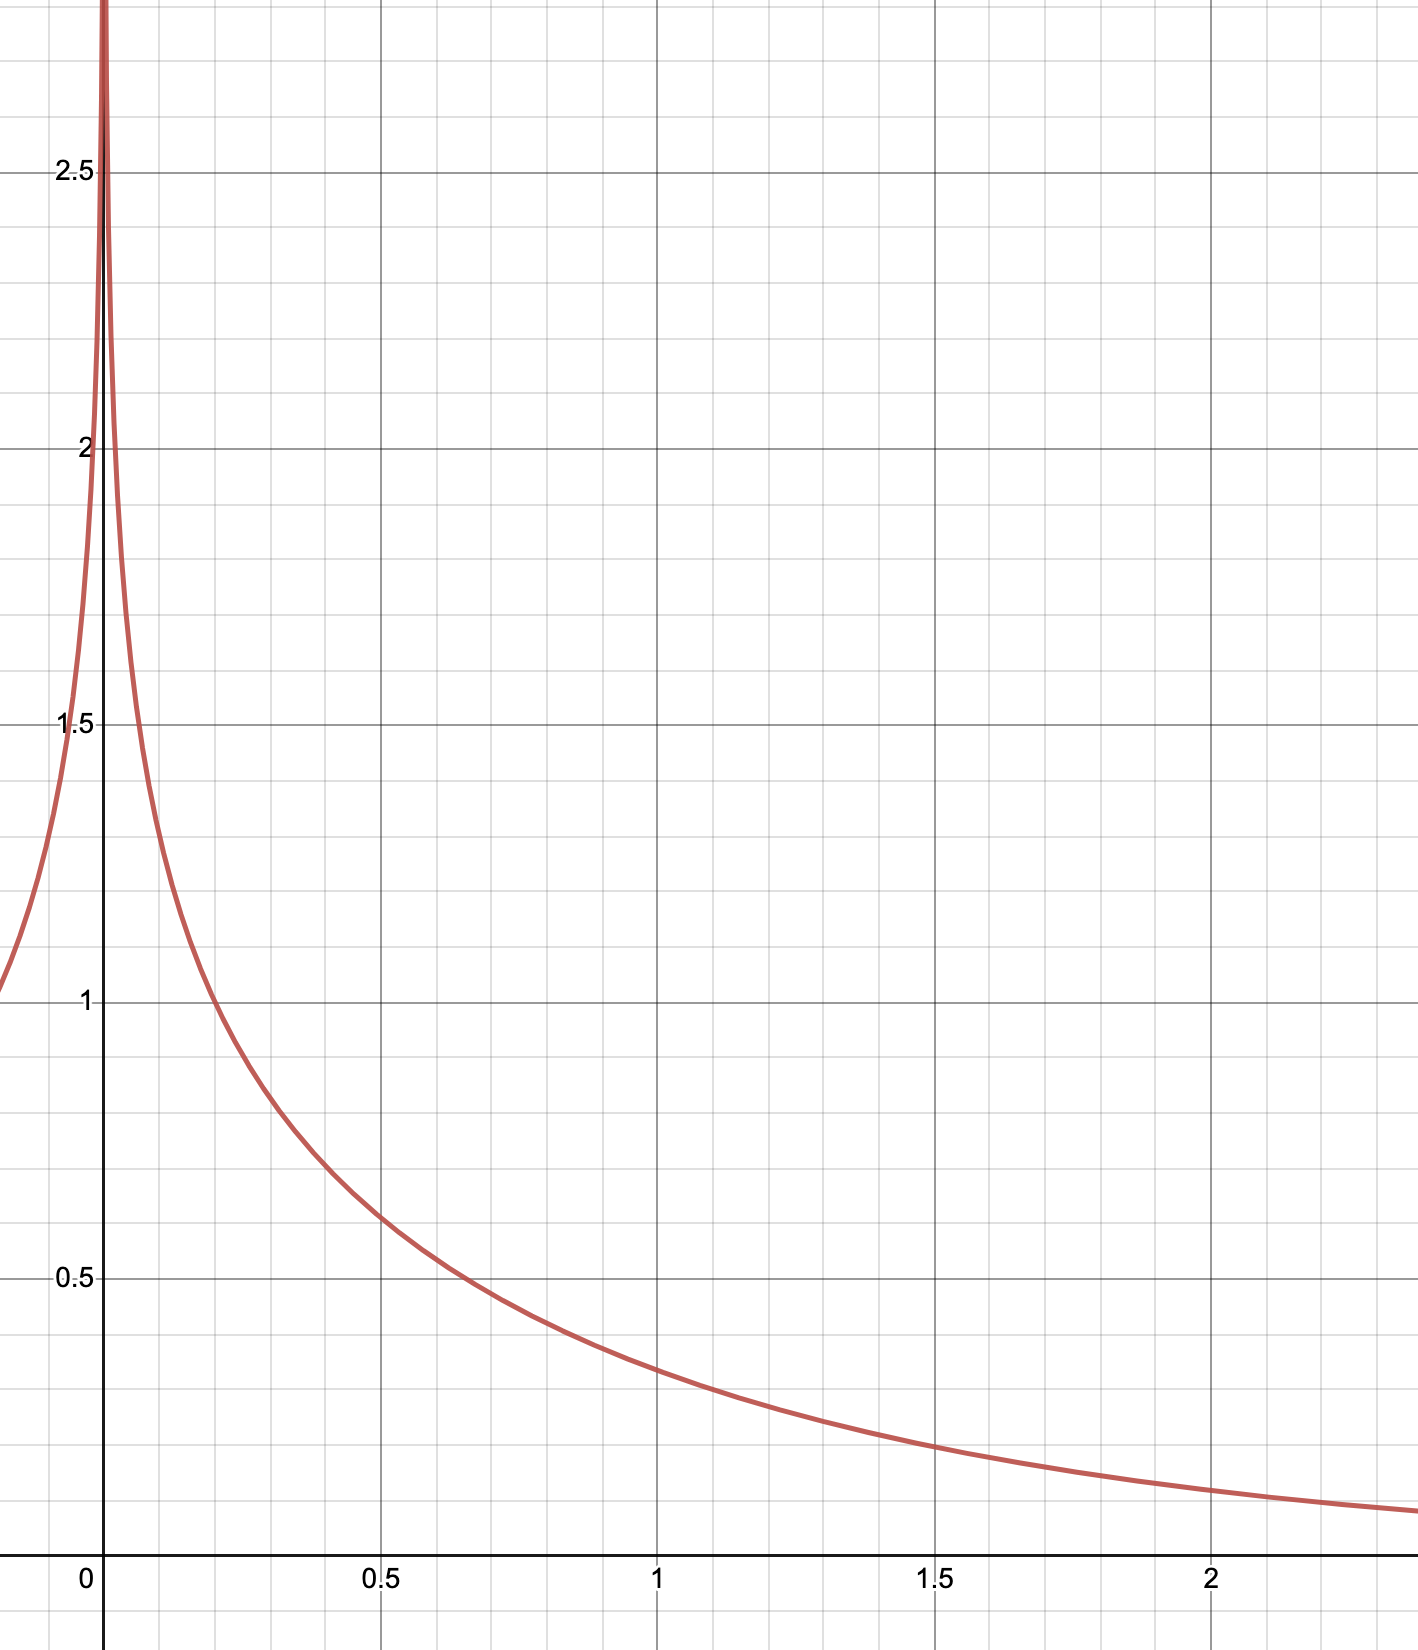
\includegraphics[width=0.5\textwidth]{./minsumapprox.png}
\end{center}
\end{frame}

\begin{frame}[label={sec:org9aeebc2}]{Min-sum approximation}
Small values dominate, so \(f(|l_1|) + f(|l_2|) =
f(\min{(|l_1|, |l_2|)})\). Translating back to our original formula,
$$|l_{ext,0}| = f(f(l_1) + f(l_2)) = f(f(\min{(|l_1|, |l_2|)})) =
\min{(|l_1|, |l_2|)}$$
Since \(f\) is its own inverse.
\end{frame}

\begin{frame}[label={sec:org236c83d}]{SISO Decoder for General (n, n-1) SPC Code}
Generalizes very naturally:

$$l_0 = \frac{2}{\sigma^2}r_0$$
and
$$l_{ext,0} = (\sgn{(l_1)}\sgn{(l_2)}\cdots\sgn{(l_{n-1})})\min{(|l_1|, |l_2|,
\ldots, |l_{n-1}|)}$$

\ldots{}and so on for each \(L_i\). Low-hanging optimizations here for both
the sign and the minimum operations.
\end{frame}

\section{Formalizing Linear Block Codes}
\label{sec:org2e2c8ff}

\begin{frame}[label={sec:org2f0f6fa}]{Introduction}
\begin{itemize}
\item From Wikipedia: ``A \alert{linear code} of length \emph{n} and dimension
\emph{k} is a linear subspace \emph{C} with dimension \emph{k} of the vector space
\(\mathbb{F}_q^n\) where \(\mathbb{F}_q\) is the
finite field with \emph{q} elements.''
\item More simply, a linear block code takes an input vector of bits
\(\vec{m}\), and produces \(\vec{c} = [\vec{m}~\vec{p}]\), where
\(\vec{p}\) is the \emph{parity check vector}.
\item \(\vec{m}\) is of dimension (length) \(k\), \(\vec{p}\) is of dimension
\(p\), and \(\vec{c}\) is of dimension \(n=k+p\).
\item The elements of \(\vec{p}\) are computed by XORing (adding modulo 2)
certain bits of \(\vec{m}\).
\end{itemize}
\end{frame}

\begin{frame}[label={sec:orgd4e60b8}]{Example of simple (6, 3) linear block code}
Parity computation is given by:
\begin{align*}
p_0 &= m_0 \oplus m_1\\
p_1 &= m_1 \oplus m_2\\
p_2 &= m_2 \oplus m_0\\
\end{align*}

Clearly, the rate is \(R=1/2\).
\end{frame}

\begin{frame}[label={sec:org5ecd11e}]{Generator matrices}
Clearly,
$$\begin{bmatrix} p_0 & p_1 & p_2 \end{bmatrix} = \begin{bmatrix} m_0
& m_1 & m_2 \end{bmatrix} \begin{bmatrix}
1&0&1\\1&1&0\\0&1&1\end{bmatrix}$$

To get the full systematic codeword, tack on \(I_3\):
$$\begin{bmatrix} m_0 & m_1 & m_2 & p_0 & p_1 & p_2 \end{bmatrix} = \begin{bmatrix} m_0
& m_1 & m_2 \end{bmatrix} \underbrace{\begin{bmatrix}
1&0&0&1&0&1\\0&1&0&1&1&0\\0&0&1&0&1&1\end{bmatrix}}_{G}$$
This matrix is known as the generator matrix for the code: \(G =
[I_k~P]\). It has rank \(k\), and its rows form the basis for the code
space.
\end{frame}

\begin{frame}[label={sec:orgfb90911}]{Parity check matrix}
\begin{itemize}
\item Given by \(H = [P^T~I_{n-k}]\), a \((n-k)\times n\) matrix.
\end{itemize}
$$\underbrace{\begin{bmatrix}
1&1&0&1&0&0\\0&1&1&0&1&0\\1&0&1&0&0&1\end{bmatrix}}_{H} \begin{bmatrix}
m_0 \\ m_1 \\ m_2 \\ p_0 \\ p_1 \\ p_2\end{bmatrix} = \begin{bmatrix}
0\\0\\0\end{bmatrix}$$

\begin{itemize}
\item In general, given a codeword, \(Hc^{T} = 0\).
\end{itemize}
\end{frame}


\begin{frame}[label={sec:org04653ba}]{Exercise}
Construct the generator matrix \(G\) and parity check matrix \(H\) for the
\(n=3\) repetition code.

Bonus: do the same for the (7, 4) Hamming code.
\end{frame}

\begin{frame}[label={sec:org28a358b}]{Solution}
$$G = \begin{bmatrix} 1&1&1\end{bmatrix}$$
$$H = \begin{bmatrix} 1&0&1\\0&1&1\end{bmatrix}$$
\end{frame}

\section{Low Density Parity Check Codes}
\label{sec:org8234c74}

\begin{frame}[label={sec:org62079db}]{Some of the keywords should now make sense}
\begin{itemize}
\item LDPC codes are linear block codes with a very sparse parity check
matrix \(H\).
\item That is, \(\mathtt{popcount(H)} << n(n-k)\).
\end{itemize}
\end{frame}

\begin{frame}[label={sec:org3efe749}]{Tanner Graphs and Parity Check Matrices}
\alert{Important:} any one row of \(H\) that is, each check node corresponds
to a \alert{single parity check code}.
\begin{center}
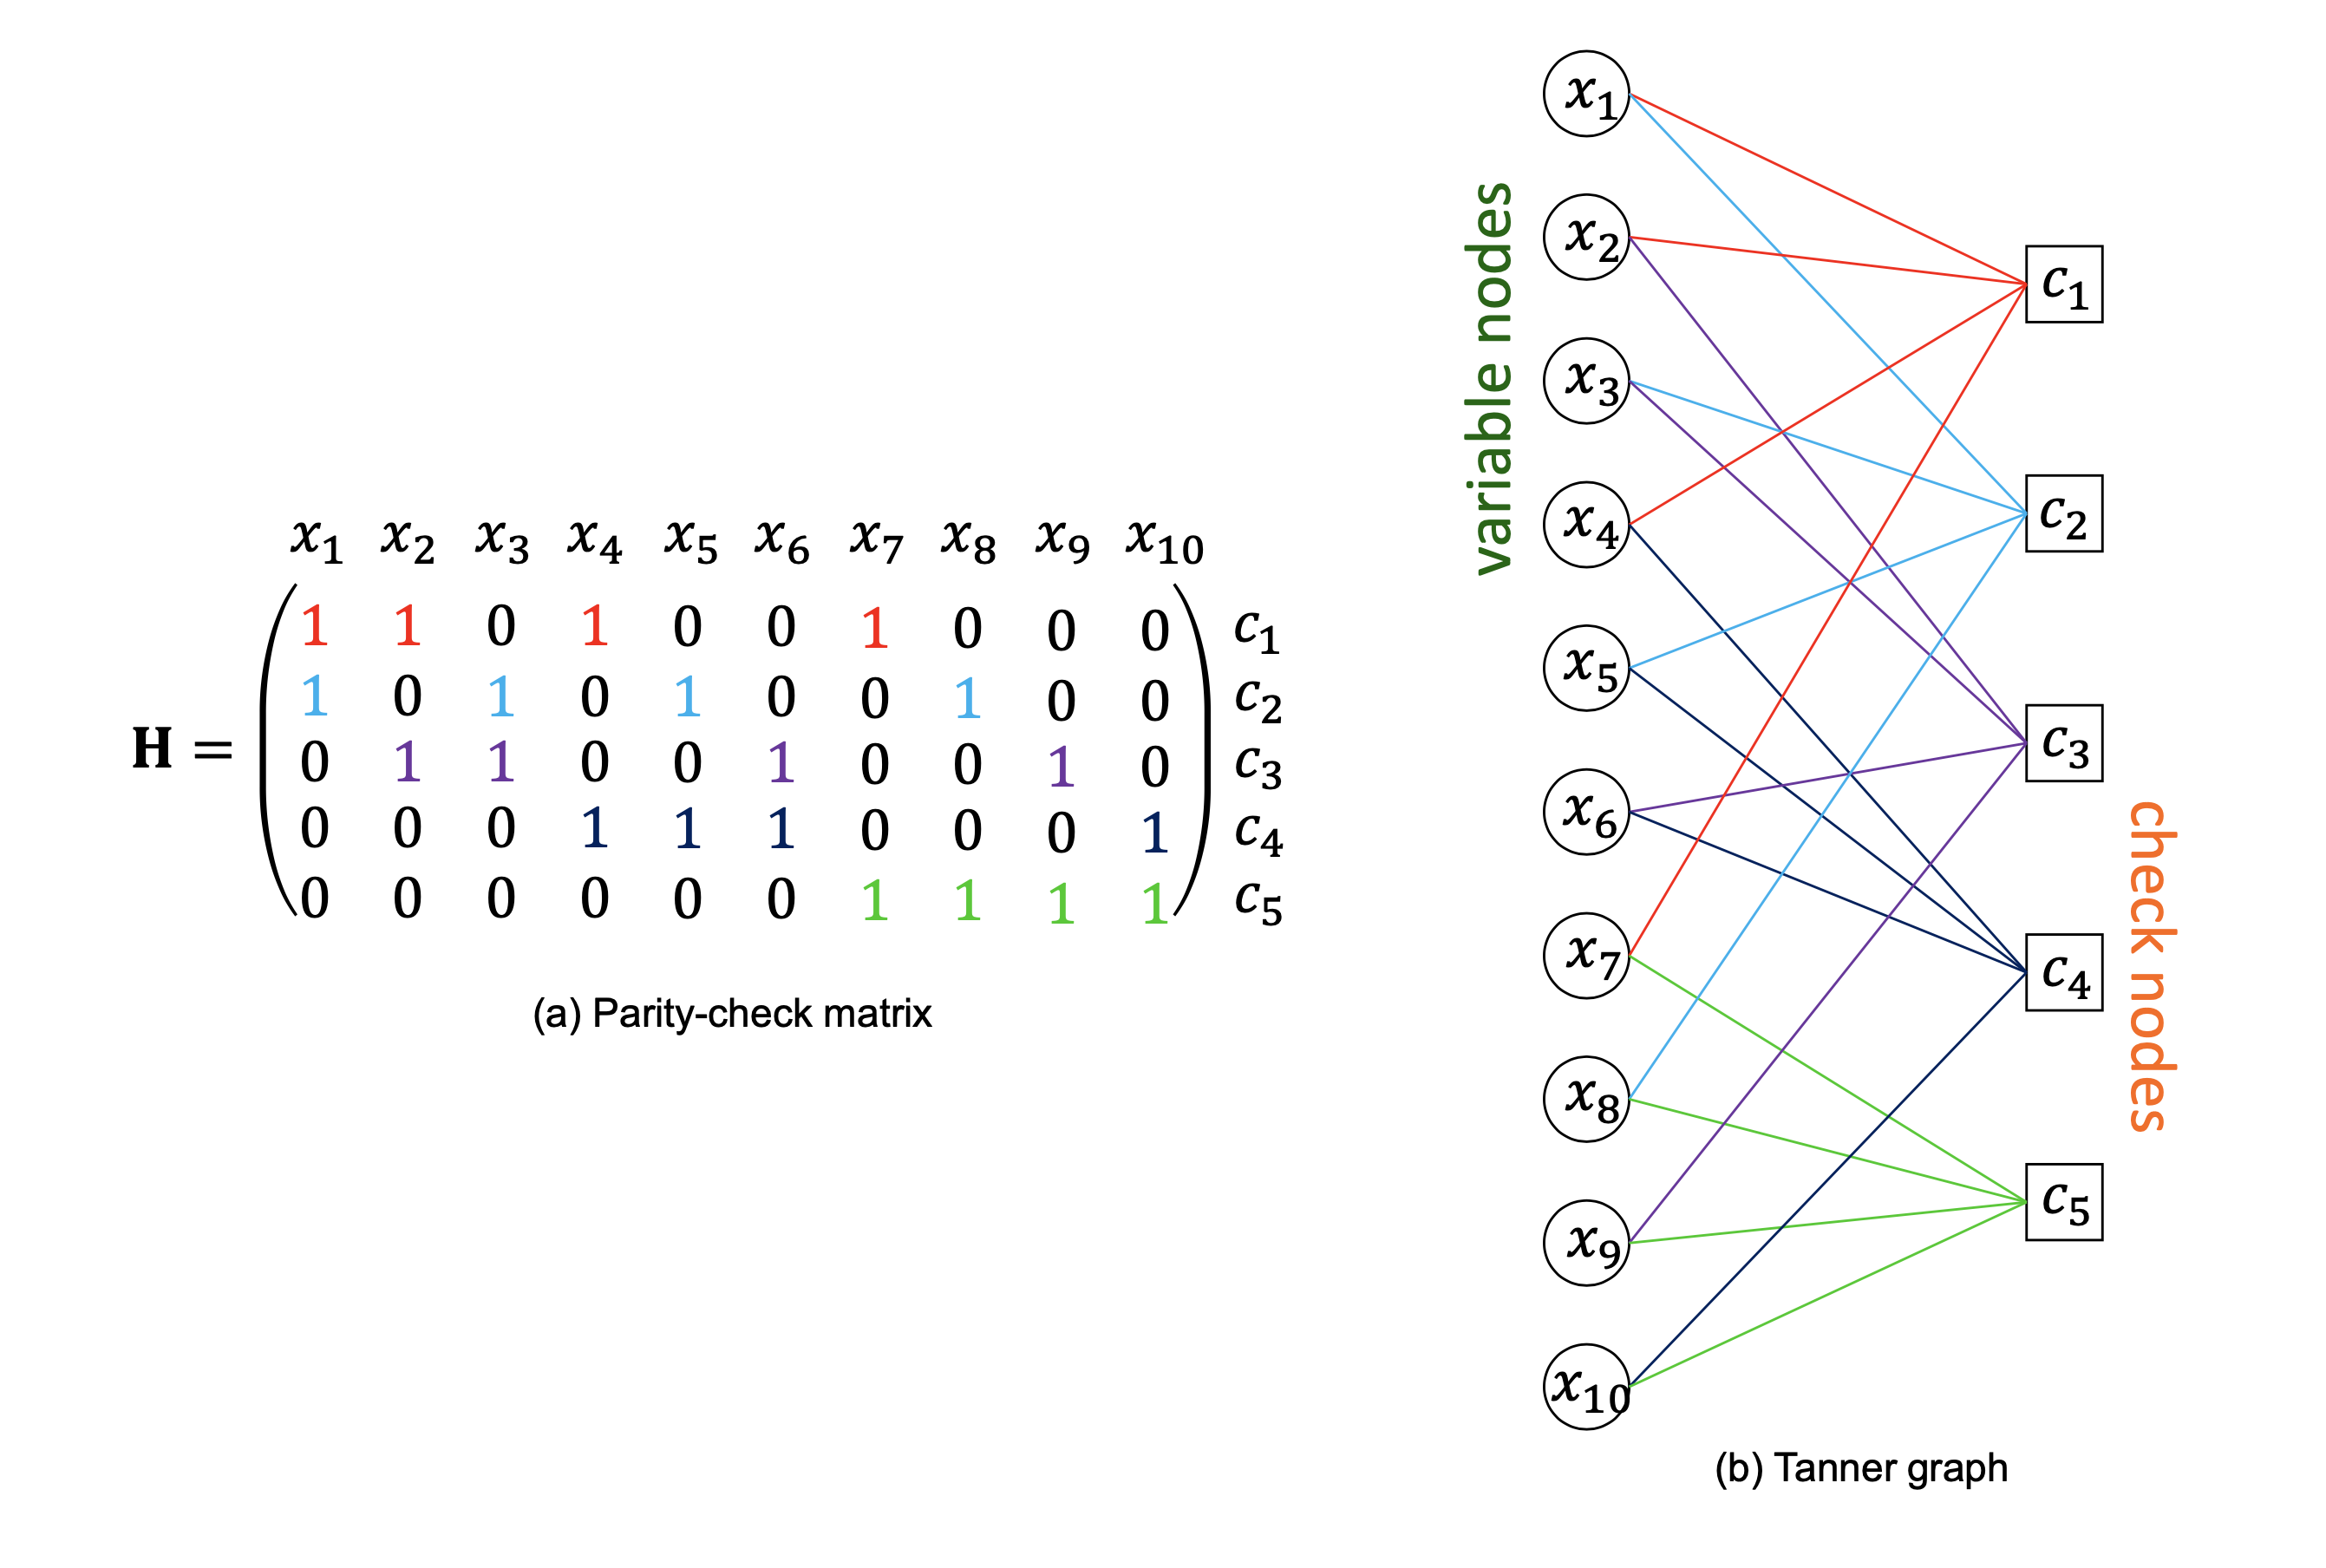
\includegraphics[width=0.8\textwidth]{./tanner.png}
\end{center}
\end{frame}

\begin{frame}[label={sec:org01dda87}]{Code Generation and Encoding}
\begin{itemize}
\item Isn't terribly interesting, and we may come back to it later.
\item Fundamentally the same idea as encoding any linear block code: a
matrix multiplication (alternately, using the parity check matrix to
figure out which bits to XOR).
\item To optimize code performance, encoding complexity, memory footprint,
a ``base matrix'' is carefully selected, then expanded in a certain
way using circulant matrices to get the parity check matrix.
\item The really interesting part of LDPC is the decoding algorithm.
\end{itemize}
\end{frame}


\begin{frame}[label={sec:org9eef026}]{LDPC Decoding}
\begin{itemize}
\item SISO
\item Iterative, belief propagation algorithm
\item Uses the min-sum approximation from earlier
\item For SISO decoding, recall that we want
$$L_i = \log{\frac{P(c_i=0|\vec{r})}{P(c_i=1|\vec{r})}}$$
that indicates the strength of the ``belief'' that bit \(c_i\) of the
codeword is (say) 0.
\end{itemize}
\end{frame}


\begin{frame}[label={sec:orgbb9138c}]{Plan: use the Tanner graph}
\begin{itemize}
\item Variable nodes (LHS) are connected to check nodes (RHS).
\item Pass extrinsic information through the edges of the graph, so all
the nodes ``work together'', adding their knowledge.
\item Four steps of the decoding algorithm:
\begin{enumerate}
\item Initialization
\item Check-node processing
\item Variable-node processing
\item If syndrome is not zero or maximum iterations not reached, GOTO 2.
\end{enumerate}
\end{itemize}
\end{frame}

\begin{frame}[label={sec:orgebd0ed8}]{Visualization in the Tanner Graph}
Initialize all the variable nodes with their channel (intrinsic) LLR \(l_i\).
\begin{center}
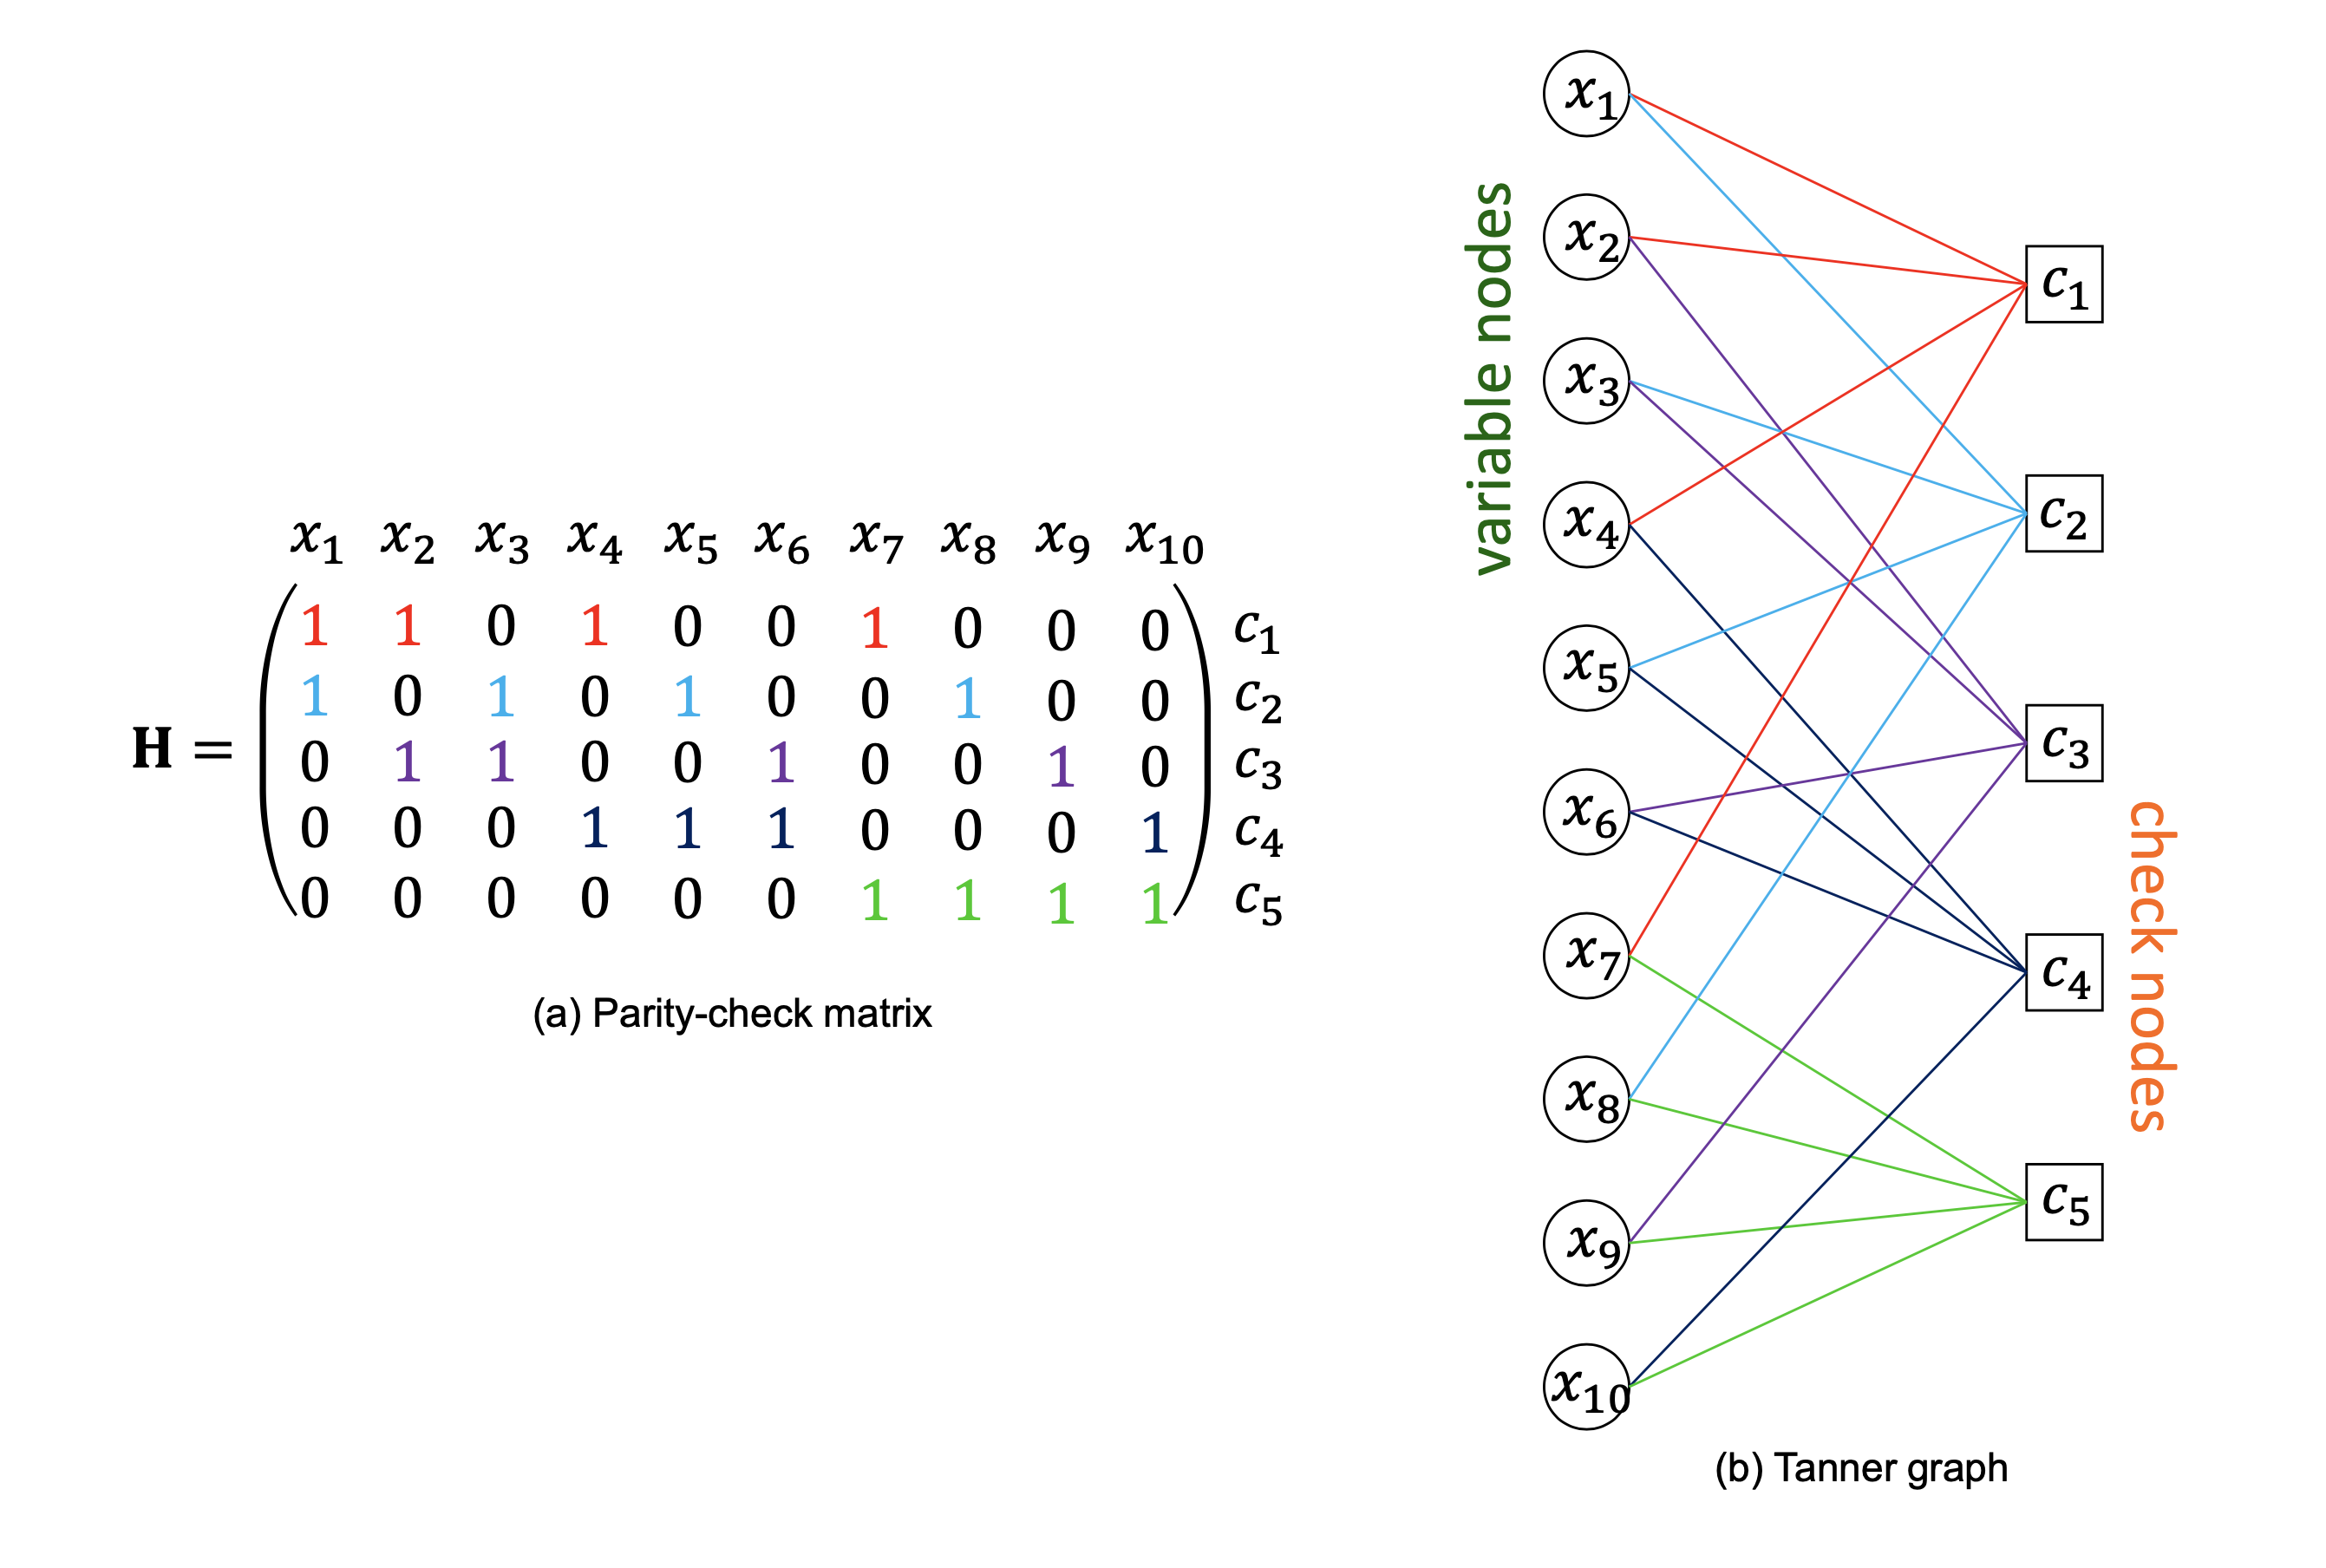
\includegraphics[width=0.8\textwidth]{./tanner.png}
\end{center}
\end{frame}

\begin{frame}[label={sec:orgb8b568b}]{Check-node processing}
\begin{center}
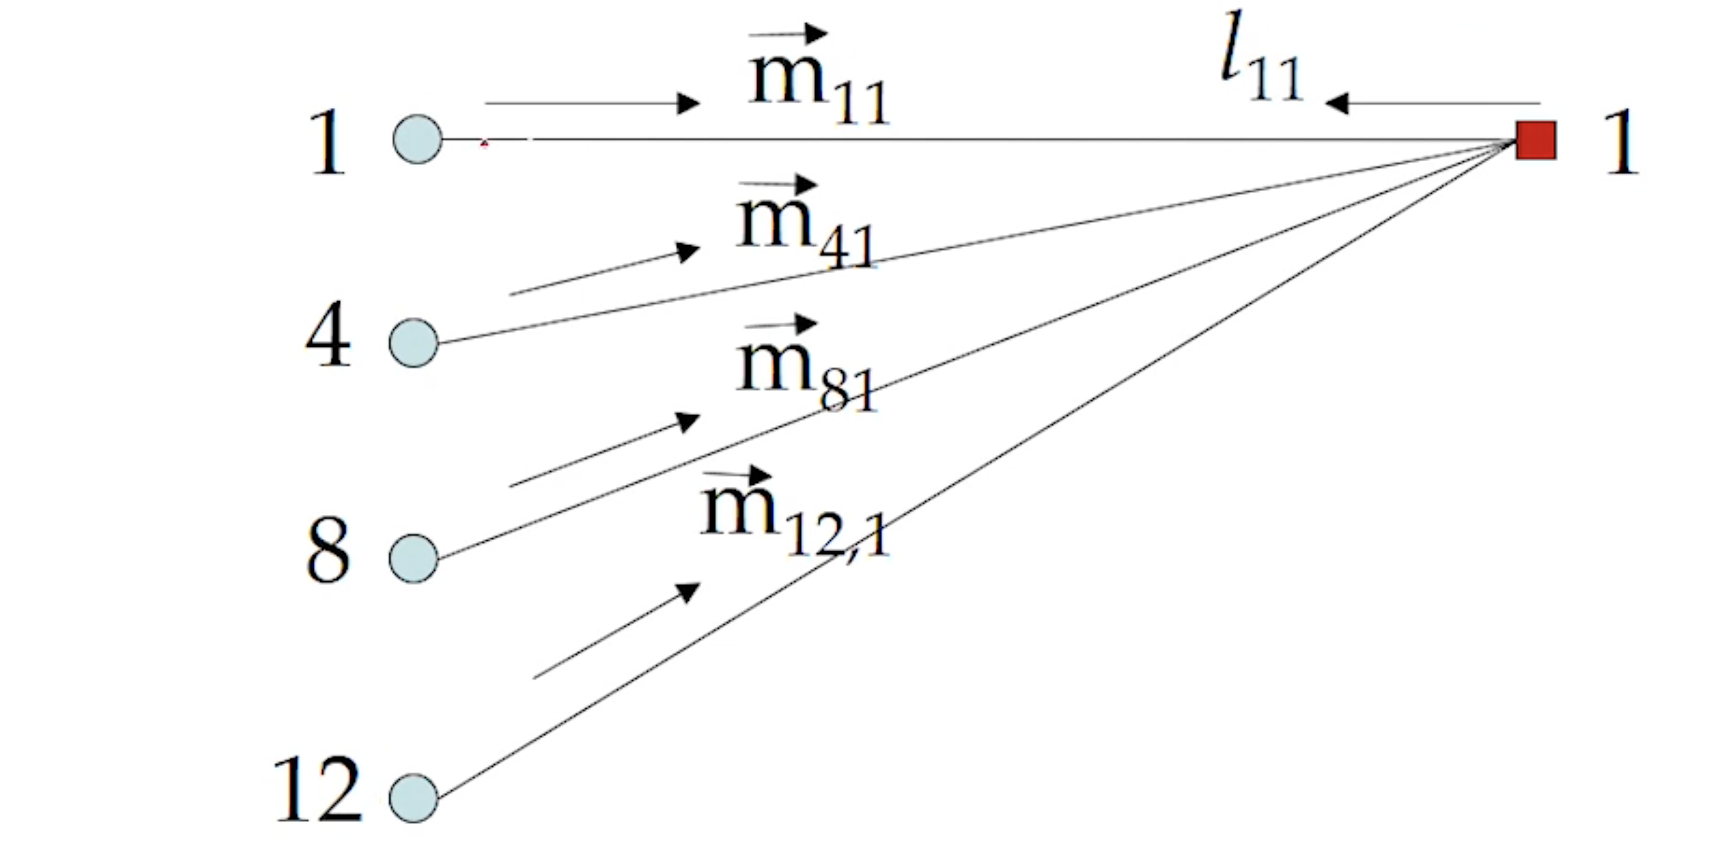
\includegraphics[width=.9\linewidth]{./first_iter.png}
\end{center}

This is an SPC! Check node (1) (say \(\beta_1\)) will do a SISO SPC decoding.
\end{frame}

\begin{frame}[label={sec:orga67fef6}]{Variable-node processing}
\begin{center}
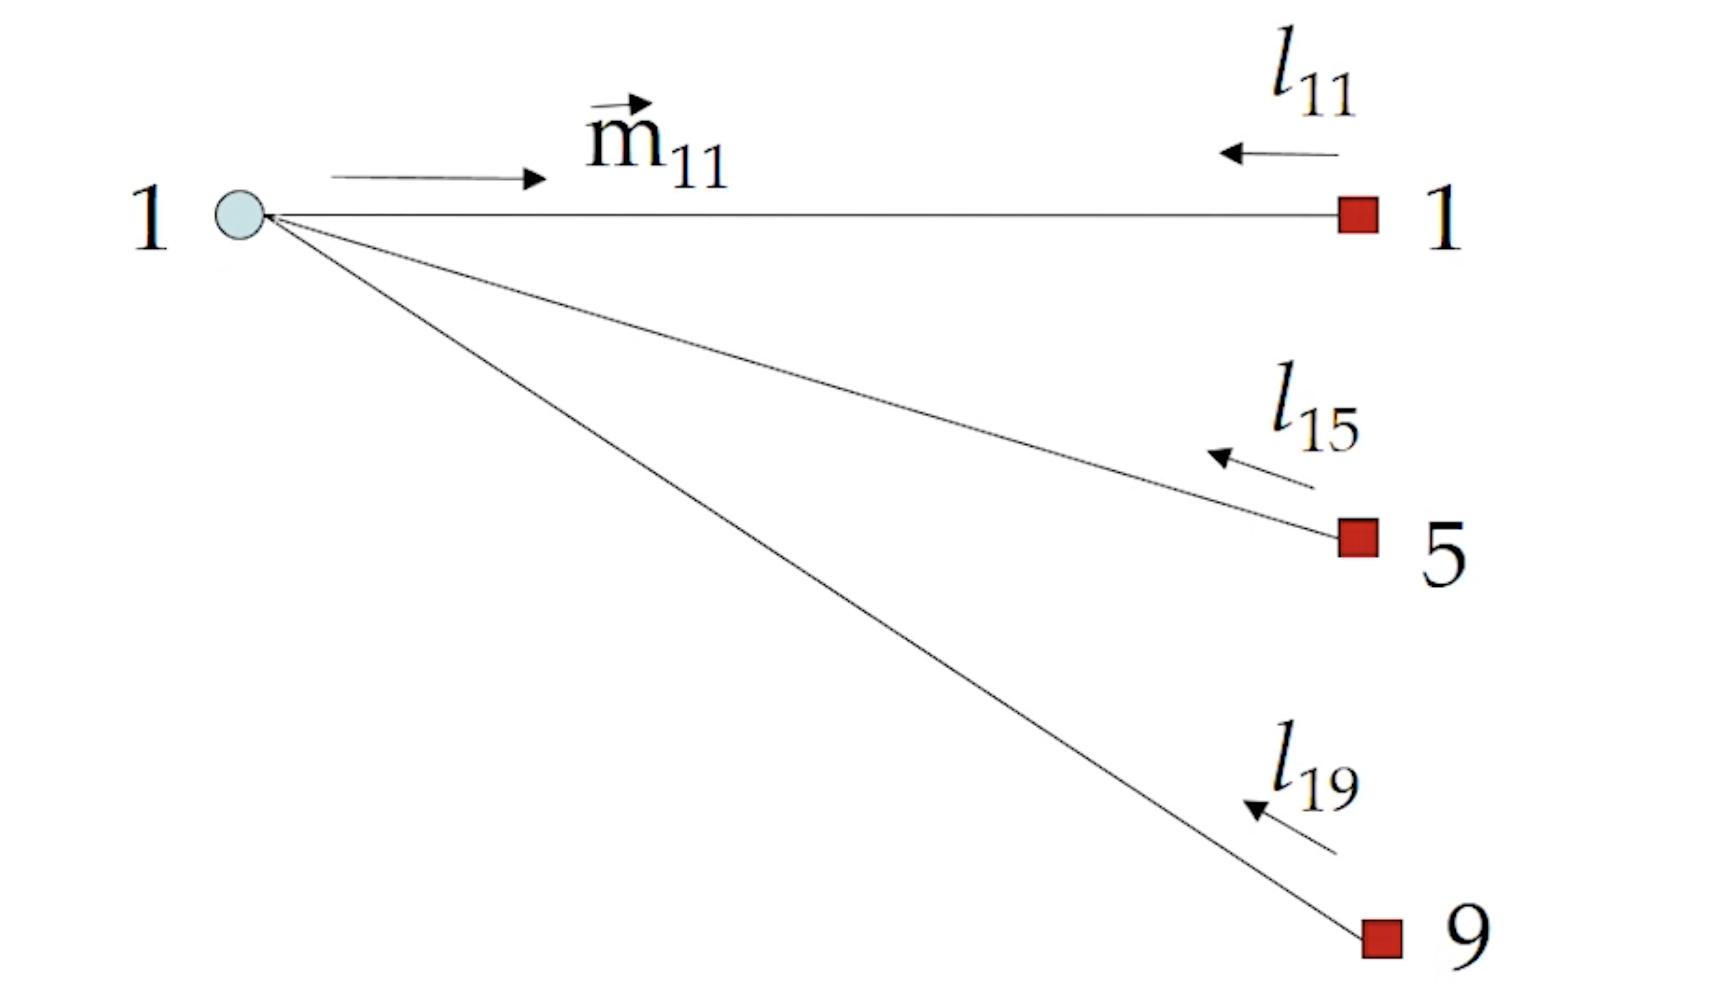
\includegraphics[width=.9\linewidth]{./next_iter.png}
\end{center}
Each check node returns the \emph{extrinsic} information from the
SPC computation for each variable node (say \(\alpha_i\)). This forms a
repetition code!
\end{frame}

\begin{frame}[label={sec:org92b3904}]{Some properties}
\begin{itemize}
\item More iterations is better
\item Using the min-sum approximation causes a degradation in error-rate
performance, but makes SISO SPC check node decoders very simple.
\item Small cycles in the Tanner graph (low girth) can ruin performance
for iterative decoding.
\item Characterizing performance of LDPC codes requires ``density
evolution'' analysis.
\end{itemize}
\end{frame}

\begin{frame}[label={sec:org85735ae}]{Thanks for coming!}
\tiny From \url{https://www.inference.org.uk/mackay/codes/gifs/}
\begin{center}
\animategraphics[loop, width=0.4\textwidth]{5}{./gif/ldpc_decode-}{0}{15}
\end{center}
\end{frame}
\end{document}